% !Mode:: "TeX:UTF-8"
\part{Laser Localization and Mapping}  
\thispagestyle{empty}  
\chapter{Basic Point Cloud Processing}  
\thispagestyle{empty}  

From this section onwards, we will spend some time introducing the laser SLAM system. Laser sensors are one of the most important sensors in autonomous driving and robotics applications. We can use devices such as lasers, inertial navigation, and satellite navigation to build a complete high-precision mapping and localization application. However, not all researchers are familiar with these sensors. Laser sensors themselves can be categorized into various types, such as single-line, multi-line, mechanical, and solid-state, each with vastly different processing methods.  

In this chapter, we will start with basic point cloud processing algorithms and gradually introduce readers to a complete laser SLAM system, including both 2D and 3D aspects. Compared to inertial navigation data or image data, laser data is relatively simple: lasers only detect the three-dimensional structure of objects and do not involve the kinematics of objects or complex projection processes. Mathematically, a $\mathbb{R}^3$ space can well describe the measurement data from a laser.  

However, at the computational level, we still encounter some issues. The most fundamental of these is \textbf{how to define spatial adjacency}. This problem is referred to as the \textbf{Nearest Neighbour (NN)} problem. We will find that the \textbf{nearest neighbour} between points is the foundation of many algorithms, yet this seemingly simple task can be approached in many different ways computationally. We could use the simplest arrays to represent point clouds, but that would fail to capture the relationships between points. To facilitate adjacency calculations, we also explore more complex \textbf{tree structures}, which are more efficient than traditional methods in handling nearest neighbour problems. Many point cloud registration algorithms require calculating the error between a point and its surrounding points based on some metric. This metric could be the Euclidean distance between points, the \textbf{point-to-line} or \textbf{point-to-plane} distance, or some \textbf{statistically meaningful} metric. Different metric selection methods lead to different algorithms, but they all share common theoretical foundations. For example, pre-dividing space according to some \textbf{criterion} and then building an \textbf{indexed} data structure to facilitate the search for point-to-point adjacency relationships. The methods of division here are diverse, ranging from simple grid-based approaches to planes, spheres, interfaces, etc., giving rise to numerous algorithms. We will introduce the important ones to the readers.  

In this chapter, we will first cover the basic algorithms for point clouds, including how to represent point clouds, how to describe the mathematical model of a laser sensor, how to find the neighbouring points of a given point, how to fit simple geometric shapes to a set of points, and so on. The next two chapters will build upon this content to develop 2D and 3D registration methods.  

\includepdf[width=\textwidth]{art/ch5.pdf}

\section{Mathematical Models of Laser Sensors and Point Clouds}  
\subsection{Mathematical Model of Laser Sensors}  
\begin{figure}[!htp]  
	\centering  
	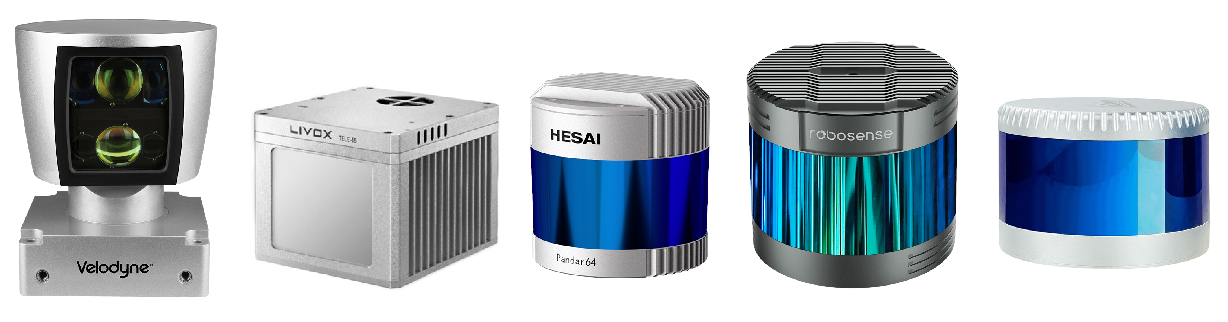
\includegraphics[width=0.8\textwidth]{resources/basic-point-cloud/lidars.pdf}  
	\caption{Various radar models used in autonomous driving. From left to right: Velodyne HDL-64, DJI Livox, Hesai, RoboSense, and LeiShen.}  
	\label{fig:lidars}  
\end{figure}  

Lidar is the most important sensor in autonomous driving. It provides high-precision distance measurement information but remains quite expensive. To this day, there is still intense debate over whether Lidar should be used in autonomous vehicles. Autonomous driving employs various models of Lidar, some of which are listed in Figure~\ref{fig:lidars}. Broadly speaking, Lidar used in autonomous driving can be divided into two types: \textbf{mechanical spinning Lidar} and \textbf{solid-state Lidar}\footnote{Hereafter, we will consistently use the term \textbf{radar} to refer to laser ranging sensors, though this may cause some ambiguity in expression. The \textbf{radar} mentioned here is a transliteration of the English term "Lidar," which stands for Light Detection and Ranging. In the context of autonomous driving, Lidar is often abbreviated as radar. However, in other fields, radar refers to Radio Detection and Ranging, or Radar for short. In Chinese, both Lidar and Radar can be referred to as radar, while in English, they are distinct terms. Notably, autonomous driving also uses millimeter-wave radar, often called Radar. In this book, radar uniformly refers to Lidar, not millimeter-wave radar.}.  

\begin{enumerate}  
	\item \textbf{Mechanical spinning Lidar} can be viewed as a column of laser probes rotating at a fixed frequency. Each probe can quickly measure the distance to external objects.  
	Each full rotation of the probes completes one scan of the surrounding environment. Lidar can be further categorized by the number of lines, common configurations include single-line, 4-line, 8-line, 16-line, 32-line, 64-line, 80-line, and 128-line. The higher the number of lines, the more points are captured per scan, and the richer the information. However, even after multiple price reductions, high-line-count spinning Lidar (32-line and above) remains a very expensive sensor, often costing several times the price of the vehicle itself\footnote{Based on 2021 prices.}.  
	\item \textbf{Solid-state Lidar} is a rapidly developing new type of Lidar in recent years. Unlike mechanical Lidar, solid-state Lidar does not perform 360-degree scans; it can only detect 3D information within a field of view of about 120 degrees. They are very similar to RGB-D cameras (the two are also similar in principle). Most solid-state Lidar systems have a field of view ranging from 60 to 120 degrees but are cheaper and can achieve image-like scanning. In terms of equivalent line count, solid-state Lidar can even achieve effects comparable to 200 lines or more, though solid-state Lidar does not necessarily scan along horizontal lines—some have unique scanning patterns.  
\end{enumerate}  

Spinning Lidar and solid-state Lidar each have their pros and cons. The 360-degree scanning capability of spinning Lidar is highly advantageous for localization and mapping, as the panoramic view ensures that the entire road segment can be mapped in a single pass, and point cloud localization is less susceptible to occlusion. When using solid-state Lidar, multiple units are often combined to achieve a similar panoramic effect. However, spinning Lidar has clear disadvantages in terms of cost and lifespan, and in the near term, it still does not meet automotive-grade or consumer-level price requirements. In contrast, solid-state Lidar can easily achieve costs in the range of several thousand yuan, meeting safety and lifespan requirements at the expense of some field of view (which can be compensated for by using multiple units), and has gained many supporters in recent years. Some high-end vehicle models have already begun equipping solid-state Lidar as part of their perception systems.  

The debate over whether autonomous driving should use Lidar has never ceased. Some believe L4 autonomous driving cannot do without Lidar, while others vehemently argue that Lidar is a burden on vehicles. There are also moderates who are indifferent to the type of sensor, focusing only on functionality and cost. For L4, the early development of autonomous driving primarily relied on mechanical spinning Lidar, so current technical solutions exhibit some degree of path dependence on spinning Lidar. Path dependence refers to the phenomenon where early algorithms and research were tailored to an initial solution, often without regard to cost. Without causing significant issues, there is little incentive to change this solution over time. However, viewed years later, this solution may not necessarily be the best in practice.  

This book does not intend to engage in debates about sensors but focuses solely on introducing their principles and algorithms. Compared to visual and IMU sensors, the measurement of a single laser probe is extremely simple: it merely measures the distance to a point in space, denoted as $r$. Of course, the laser probe itself can be mounted on the vehicle at a certain tilt angle, allowing the spatial position of the endpoint to be determined. This model is called the RAE (Range, Azimuth, Elevation) model, as shown in Figure~\ref{fig:RAE}.  

\begin{figure}[!htp]  
	\centering  
	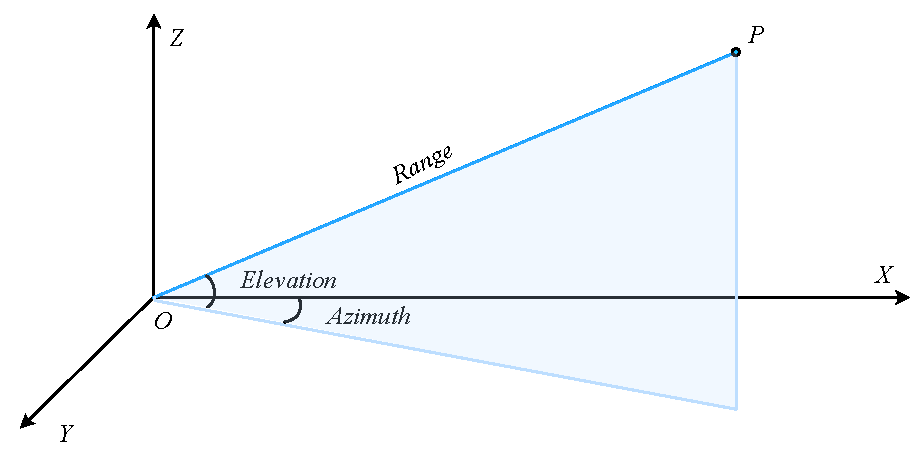
\includegraphics[width=0.8\textwidth]{resources/basic-point-cloud/RAE.pdf}  
	\caption{RAE model for single-point measurement}  
	\label{fig:RAE}  
\end{figure}  

Let the distance be $r=\text{Range}$, the azimuth angle be $A=\text{Azimuth}$, and the elevation angle be $E=\text{Elevation}$. These angles are similar to Euler angles. Based on geometric relationships, the position of $\bm{P}$ in the radar reference frame can easily be derived:  
\begin{equation}\label{key}  
	\bm{P} = \left[r \cos E \cos A, r \cos E \sin A, r \sin E \right] ^\top.  
\end{equation}  

Conversely, $r, A, E$ can be calculated from $\bm{P}=[x,y,z]^\top$:  
\begin{equation}\label{key}  
	\begin{aligned}  
		r &= \sqrt{x^2 + y^2 + z^2}, \\  
		A &= \arctan(y/x), \\  
		E &= \arcsin(z/r).  
	\end{aligned}  
\end{equation}  

These are simply conversions between Euclidean and polar coordinates, with no substantive difference. Spinning Lidar can be viewed as multiple RAE probe models fixed in elevation angle and rotating synchronously in azimuth angle.  
When the probes complete one full rotation, we obtain endpoints with azimuth angles ranging from 0 to 360 degrees. Typically, this set of points is called a \textbf{scan} because it closely resembles the scanning process of a scanner or television. Most Lidar systems can scan the surrounding environment at frequencies of 10 Hz or higher. If such a probe has only one line, it is a single-line Lidar, usually mounted horizontally. Multi-line Lidar can be seen as composed of multiple single-line Lidar units arranged vertically in a column, rotating at a fixed frequency. After one full scan, the multi-line Lidar produces a point cloud that fully reflects the three-dimensional structure within a certain distance. For a single probe, $E$ can be considered fixed, $A$ changes at a constant speed, and only $r$ is derived from actual measurements. This property can be leveraged to compress Lidar data—recording time and distance is simpler than recording Cartesian coordinates (i.e., the $XYZ$ data of the point cloud).  

In addition to distance, Lidar can also carry additional data. For example, multi-line Lidar can record the timestamp, reflectivity, and line number (which line the point belongs to) for each point. This information, particularly reflectivity, can be used in various practical scenarios, such as extracting road markings based on reflectivity or identifying the ground using line numbers. Basic point cloud algorithms, such as nearest neighbor and fitting algorithms, rely solely on Cartesian coordinate position data. Unless otherwise specified, the point clouds discussed hereafter refer to those containing only positional information. However, in visualization, point clouds may be rendered based on height or reflectivity.

\subsection{Representation of Point Clouds}  
\textbf{Point cloud}, in its most literal sense, refers to a set of points scattered in space. The term "\textbf{cloud}" inherently discards the relationships between points. These points are merely Cartesian coordinates in Euclidean space and carry no additional information. Do these points form a mesh? Do certain points constitute a triangle? The point cloud structure does not include such extra details.  

Point clouds are the most fundamental way to represent 3D structures and are the primary data format output by most laser sensors. If we wish to extract additional information from a point cloud, we must employ supplementary data structures to express these relationships. For instance, many algorithms require answering questions like: Which point is the nearest to a given point? What shape do this point and its neighboring points collectively form? To achieve such functionality, additional data structures must be introduced—this is the focus of this section.  

The content of this chapter overlaps with many books on 3D point clouds. Readers may also refer to similar textbooks, such as \cite{Magnusson2009, GuoHao2019}. As a book aimed at SLAM practitioners, we emphasize point cloud processing for laser sensors rather than discussing generic point cloud processing broadly. We will introduce some usage of the PCL library \cite{Rusu2011}, and for key algorithms, we also provide handwritten implementations along with performance comparisons to their PCL counterparts.  

The simplest and most primitive way to represent a point cloud is as an array: just store the points in an array. This can be easily implemented using `std::vector` in C++. Of course, as mentioned earlier, point clouds can also carry additional information, such as reflectivity, the line number (for multi-line Lidar), or RGB color data. Point clouds from RGB-D cameras may also store the row and column indices of each point in the image. Therefore, a more convenient approach is to define a point cloud structure and use a templated container to store it. If you need to store other information, such as the global position and orientation of the entire point cloud, you can define your own point cloud data structure.  

We illustrate the basics of reading, writing, and visualizing point clouds through a program example, giving readers an intuitive understanding. We have prepared two files for readers: a single-scan point cloud and a map point cloud file, located at `data/ch5/map_example.pcd` and `scan_example.pcd`, respectively. Readers can directly view these files using the `pcl_viewer` command:  
\begin{lstlisting}[language=sh,caption=Terminal input:]  
pcl_viewer ./data/ch5/map_example.pcd  
\end{lstlisting}  

We will also introduce other representation methods later. The example map and scan data are shown in Figure~\ref{fig:pcd-example}. The left point cloud depicts a small "L"-shaped scene consisting of a central building and surrounding greenery, while the right shows data from a single scan. By stitching multiple scans together, we can reconstruct the full map, whereas a single scan clearly contains far fewer points.  

\begin{figure}[!htp]  
	\centering  
	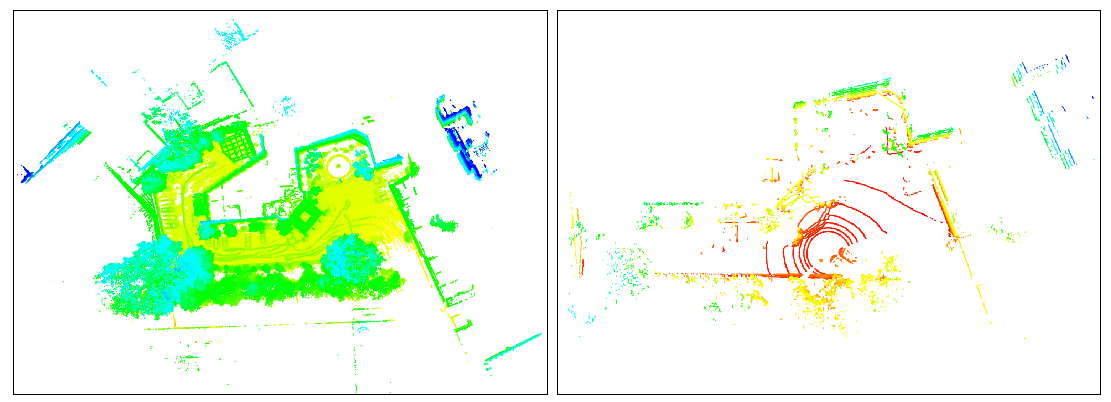
\includegraphics[width=1.0\textwidth]{resources/basic-point-cloud/pcd-example.pdf}  
	\caption{Example data of a point cloud map and a single scan.}  
	\label{fig:pcd-example}  
\end{figure}  

Below, we demonstrate how to read and visualize a point cloud, serving as a basic tutorial for PCL.  
\begin{lstlisting}[language=c++,caption=src/ch5/point\_cloud\_load\_and\_vis.cc]  
int main(int argc, char** argv) {  
	// .. Omitted parameter checking  
	// Load the point cloud  
	PointCloudType::Ptr cloud(new PointCloudType);  
	pcl::io::loadPCDFile(FLAGS_pcd_path, *cloud);  
	
	if (cloud->empty()) {  
		LOG(ERROR) << "cannot load cloud file";  
		return -1;  
	}  
	
	LOG(INFO) << "cloud points: " << cloud->size();  
	
	// Visualize  
	pcl::visualization::PCLVisualizer viewer("cloud viewer");  
	pcl::visualization::PointCloudColorHandlerGenericField<PointType> handle(cloud, "z");  // Color by height  
	viewer.addPointCloud<PointType>(cloud, handle);  
	viewer.spin();  
	
	return 0;  
}  
\end{lstlisting}  

Since data I/O and visualization are handled by existing PCL modules, we only need to call its functions. After compilation, readers can also use the program to view point clouds:  

\begin{lstlisting}[language=sh, caption=Terminal input:]  
bin/point_cloud_load_and_vis --pcd_path ./data/ch5/map_example.pcd  
\end{lstlisting}  

Most programs supporting 3D display can render point clouds effectively. Later, we will continue using 3D graphical interfaces to showcase point cloud registration results.

\subsection{Packet Representation}  

In addition to raw point clouds, there are several other representation methods. Raw point clouds store the coordinates of all points, which consumes significant space. Some representations are more suitable for storage and transmission, while others provide advantageous properties for algorithmic processing. Below, we introduce a few commonly used methods.  

In LiDAR sensors, parameters such as the rotation rate of the radar and the elevation angles of each probe relative to the sensor center are known during the design or operation of the sensor. These are referred to as the \textbf{intrinsic parameters} of the LiDAR. Therefore, these parameters can be stored in a fixed configuration file, while only the runtime-varying measurements need to be recorded in the actual data. For LiDAR, the varying components typically include the detected distance and reflectivity of objects. Leveraging this property can significantly reduce the data transmission volume between the sensor and the computer. Similarly, when storing raw point cloud data, this approach can be used to save disk space instead of storing the full point cloud. This is the concept behind \textbf{data packets} (Packets).  

Most LiDAR manufacturers define their own packet formats, which vary in implementation. These packets can be transmitted and received via various communication protocols (usually network protocols such as UDP). Taking the Velodyne HDL-64S3 as an example (Figure~\ref{fig:packets-example}), let’s examine how hardware manufacturers compress point cloud data.  

\begin{figure}[!htp]  
	\centering  
	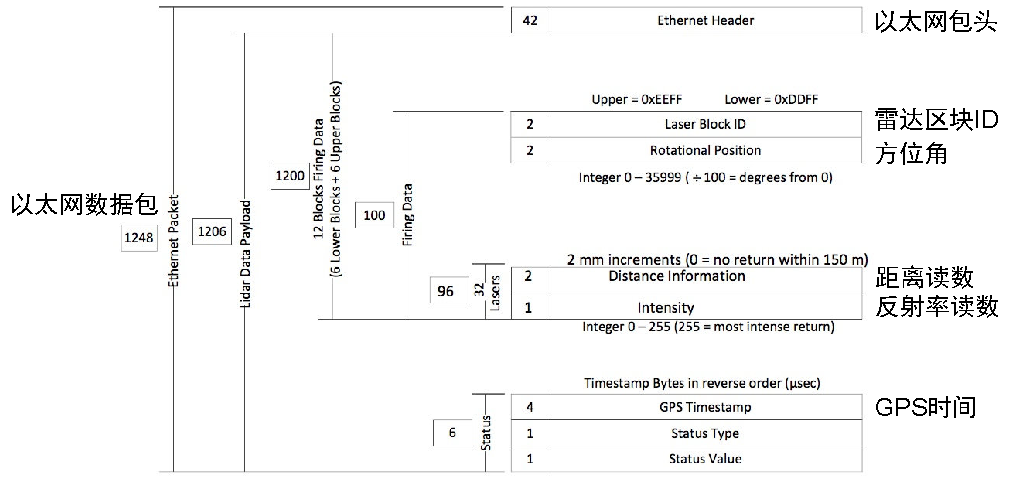
\includegraphics[width=0.8\textwidth]{resources/basic-point-cloud/packets.pdf}  
	\caption{Packet format definition for the Velodyne HDL-64S3}  
	\label{fig:packets-example}  
\end{figure}  

In the Velodyne HDL-64S3, the distance and reflectivity measurements are stored in 3 bytes, while readings from the same column share an azimuth angle and block ID. As shown, 32 readings occupy 100 bytes in total. If stored in PCL format, the positional coordinates and reflectivity of 32 scan lines would require $32 \times (4 + 4 + 4 + 1) = 416$ bytes. Clearly, storing packets is far more efficient than storing raw point clouds.  

However, in many algorithmic implementations, direct access to the coordinates of each point is often preferred. Therefore, packets are typically used as compressed data in modules such as driver software, raw sensor data handling, or map compression. Due to the variety of LiDAR brands and their differing driver implementations, manufacturers usually provide SDKs to handle the conversion between packets and point clouds. Here, we will not delve into the specifics of how each LiDAR compresses and decompresses its data.

\subsection{Bird's-Eye View and Range Image}  
Bird's-eye view (BEV) is another commonly used representation for maps, especially in outdoor environments. If we wish to express LiDAR point clouds in a grid-based format and apply grid-based algorithms for path planning, obstacle avoidance, or 2D annotations, it becomes necessary to represent the point cloud map from a top-down perspective. Of course, converting 3D information to 2D typically involves discarding some data—in this case, the height information of the point cloud.  

Since vehicles are usually horizontally positioned, the sensors mounted on them are also typically level. Under this assumption, converting an outdoor point cloud map to a bird's-eye view is straightforward, as the $x, y, z$ coordinates of the point cloud correspond directly to horizontal and vertical axes. For sensors with tilted or rotating configurations, additional ground or world coordinate system information is required. Below, we convert the point cloud from Figure~\ref{fig:pcd-example} into a bird's-eye view. The BEV is implemented using OpenCV as a 2D image. To map point cloud coordinates to image coordinates, we define a resolution $r$, which determines how many meters each pixel represents. Additionally, we ensure the image center aligns with the point cloud center, while the image dimensions depend on the $x, y$ range of the point cloud.  

Let the point cloud center be $\bm{c}=[c_x, c_y]^\top$ and the image center be $I_x, I_y$. A point with coordinates $(x, y, z)$ should map to image coordinates $(u, v)$ as follows:  

\begin{equation}\label{key}  
	\left\{  
	\begin{array}{ll}  
		u &= (x-c_x)/r + I_x, \\  
		v &= (y-c_y)/r + I_y.  
	\end{array}\right.  
\end{equation}  

The $z$-coordinate can then be represented using different colors to indicate height variations. The implementation of this process is shown below:  

\begin{lstlisting}[language=c++,caption=src/ch5/pcd\_to\_bird\_eye.cc]  
DEFINE_string(pcd_path, "./data/ch5/map_example.pcd", "Point cloud file path");  
DEFINE_double(image_resolution, 0.1, "BEV resolution");  
DEFINE_double(min_z, 0.2, "Minimum height for BEV");  
DEFINE_double(max_z, 2.5, "Maximum height for BEV");  

void GenerateBEVImage(PointCloudType::Ptr cloud) {  
	// Compute point cloud boundaries  
	auto minmax_x = std::minmax_element(cloud->points.begin(), cloud->points.end(),  
	[](const PointType& p1, const PointType& p2) { return p1.x < p2.x; });  
	auto minmax_y = std::minmax_element(cloud->points.begin(), cloud->points.end(),  
	[](const PointType& p1, const PointType& p2) { return p1.y < p2.y; });  
	double min_x = minmax_x.first->x;  
	double max_x = minmax_x.second->x;  
	double min_y = minmax_y.first->y;  
	double max_y = minmax_y.second->y;  
	
	const double inv_r = 1.0 / FLAGS_image_resolution;  
	
	const int image_rows = int((max_y - min_y) * inv_r);  
	const int image_cols = int((max_x - min_x) * inv_r);  
	
	float x_center = 0.5 * (max_x + min_x);  
	float y_center = 0.5 * (max_y + min_y);  
	float x_center_image = image_cols / 2;  
	float y_center_image = image_rows / 2;  
	
	// Generate image  
	cv::Mat image(image_rows, image_cols, CV_8UC3, cv::Scalar(255, 255, 255));  
	
	for (const auto& pt : cloud->points) {  
		int x = int((pt.x - x_center) * inv_r + x_center_image);  
		int y = int((pt.y - y_center) * inv_r + y_center_image);  
		if (x < 0 || x >= image_cols || y < 0 || y >= image_rows || pt.z < FLAGS_min_z || pt.z > FLAGS_max_z) {  
			continue;  
		}  
		
		image.at<cv::Vec3b>(y, x) = cv::Vec3b(227, 143, 79);  
	}  
	
	cv::imwrite("./bev.png", image);  
}  
\end{lstlisting}  

Now run:  
\begin{lstlisting}[caption=Terminal input:]  
bin/pcd_to_bird_eye --pcd_path ./data/ch5/map_example.pcd  
\end{lstlisting}  

We assume the point cloud is horizontally aligned and map the $X$ and $Y$ axes to the image. The initial part of the code determines the image boundaries, and then each point's position in the image is calculated based on the specified resolution. Obstacles within a certain height range (here, 0.2 to 2.5 meters, adjustable based on vehicle height) are considered valid and projected onto the BEV, resulting in the output shown in Figure~\ref{fig:bev-example}.  

\begin{figure}[!htp]  
	\centering  
	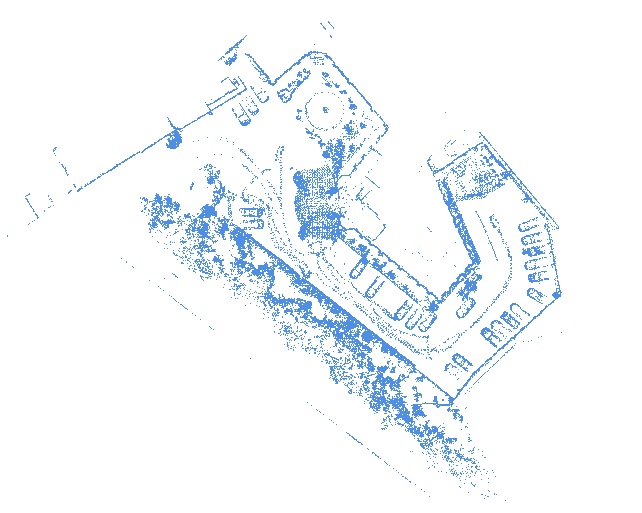
\includegraphics[width=0.6\textwidth]{resources/basic-point-cloud/bev.pdf}  
	\caption{Converting a point cloud to a bird's-eye view}  
	\label{fig:bev-example}  
\end{figure}  

Many path-planning algorithms, such as A* and D* \cite{Delling2009}, operate on grid maps, while perception or obstacle-avoidance algorithms can also use grid maps as input \cite{Sabe2004}. As seen, most obstacle information is preserved when converting point clouds to grid maps, though dynamic objects may leave smearing effects. We will discuss the probabilistic mechanism of grid maps in the 2D LiDAR SLAM chapter, which effectively mitigates the impact of dynamic objects.  

Some readers might wonder: If point clouds can be projected into a bird's-eye view, can they also be projected from other angles? While BEV is the most intuitive choice for top-down observation, similar logic can be applied to generate front or side views, which are computationally equivalent. However, another useful representation for algorithms is the \textbf{range image}.  

The concept of a range image aligns with that of RGB-D cameras. To ensure consistency between depth and color images, RGB-D cameras project point clouds into the color camera's frame. Similarly, can LiDAR point clouds be projected into a virtual camera? The answer is yes. However, since LiDAR point clouds cover a full 360-degree field of view, the resulting image is panoramic. Here, the horizontal axis represents the LiDAR's azimuth angle, while the vertical axis corresponds to the elevation angle. Alternatively, if the elevation angles for each scan line are known, the \textbf{line number} can serve as the vertical axis. Both methods produce what is known as a range image.  

As before, we provide an example to illustrate the appearance of a range image. While generating range images directly from raw LiDAR data (e.g., using block IDs or azimuth angles from packets) is more efficient, this approach depends on the specific LiDAR model. Our example uses post-processed point clouds, requiring only an additional azimuth angle calculation step.

\subsection{Bird's-Eye View and Range Image}  
Bird's-eye view (BEV) is another commonly used representation for maps, especially in outdoor environments. If we wish to express LiDAR point clouds in a grid-based format and apply grid-based algorithms for path planning, obstacle avoidance, or 2D annotations, it becomes necessary to represent the point cloud map from a top-down perspective. Of course, converting 3D information to 2D typically involves discarding some data—in this case, the height information of the point cloud.  

Since vehicles are usually horizontally positioned, the sensors mounted on them are also typically level. Under this assumption, converting an outdoor point cloud map to a bird's-eye view is straightforward, as the $x, y, z$ coordinates of the point cloud correspond directly to horizontal and vertical axes. For sensors with tilted or rotating configurations, additional ground or world coordinate system information is required. Below, we convert the point cloud from Figure~\ref{fig:pcd-example} into a bird's-eye view. The BEV is implemented using OpenCV as a 2D image. To map point cloud coordinates to image coordinates, we define a resolution $r$, which determines how many meters each pixel represents. Additionally, we ensure the image center aligns with the point cloud center, while the image dimensions depend on the $x, y$ range of the point cloud.  

Let the point cloud center be $\bm{c}=[c_x, c_y]^\top$ and the image center be $I_x, I_y$. A point with coordinates $(x, y, z)$ should map to image coordinates $(u, v)$ as follows:  

\begin{equation}\label{key}  
	\left\{  
	\begin{array}{ll}  
		u &= (x-c_x)/r + I_x, \\  
		v &= (y-c_y)/r + I_y.  
	\end{array}\right.  
\end{equation}  

The $z$-coordinate can then be represented using different colors to indicate height variations. The implementation of this process is shown below:  

\begin{lstlisting}[language=c++,caption=src/ch5/pcd\_to\_bird\_eye.cc]  
DEFINE_string(pcd_path, "./data/ch5/map_example.pcd", "Point cloud file path");  
DEFINE_double(image_resolution, 0.1, "BEV resolution");  
DEFINE_double(min_z, 0.2, "Minimum height for BEV");  
DEFINE_double(max_z, 2.5, "Maximum height for BEV");  

void GenerateBEVImage(PointCloudType::Ptr cloud) {  
	// Compute point cloud boundaries  
	auto minmax_x = std::minmax_element(cloud->points.begin(), cloud->points.end(),  
	[](const PointType& p1, const PointType& p2) { return p1.x < p2.x; });  
	auto minmax_y = std::minmax_element(cloud->points.begin(), cloud->points.end(),  
	[](const PointType& p1, const PointType& p2) { return p1.y < p2.y; });  
	double min_x = minmax_x.first->x;  
	double max_x = minmax_x.second->x;  
	double min_y = minmax_y.first->y;  
	double max_y = minmax_y.second->y;  
	
	const double inv_r = 1.0 / FLAGS_image_resolution;  
	
	const int image_rows = int((max_y - min_y) * inv_r);  
	const int image_cols = int((max_x - min_x) * inv_r);  
	
	float x_center = 0.5 * (max_x + min_x);  
	float y_center = 0.5 * (max_y + min_y);  
	float x_center_image = image_cols / 2;  
	float y_center_image = image_rows / 2;  
	
	// Generate image  
	cv::Mat image(image_rows, image_cols, CV_8UC3, cv::Scalar(255, 255, 255));  
	
	for (const auto& pt : cloud->points) {  
		int x = int((pt.x - x_center) * inv_r + x_center_image);  
		int y = int((pt.y - y_center) * inv_r + y_center_image);  
		if (x < 0 || x >= image_cols || y < 0 || y >= image_rows || pt.z < FLAGS_min_z || pt.z > FLAGS_max_z) {  
			continue;  
		}  
		
		image.at<cv::Vec3b>(y, x) = cv::Vec3b(227, 143, 79);  
	}  
	
	cv::imwrite("./bev.png", image);  
}  
\end{lstlisting}  

Now run:  
\begin{lstlisting}[caption=Terminal input:]  
bin/pcd_to_bird_eye --pcd_path ./data/ch5/map_example.pcd  
\end{lstlisting}  

We assume the point cloud is horizontally aligned and map the $X$ and $Y$ axes to the image. The initial part of the code determines the image boundaries, and then each point's position in the image is calculated based on the specified resolution. Obstacles within a certain height range (here, 0.2 to 2.5 meters, adjustable based on vehicle height) are considered valid and projected onto the BEV, resulting in the output shown in Figure~\ref{fig:bev-example}.  

\begin{figure}[!htp]  
	\centering  
	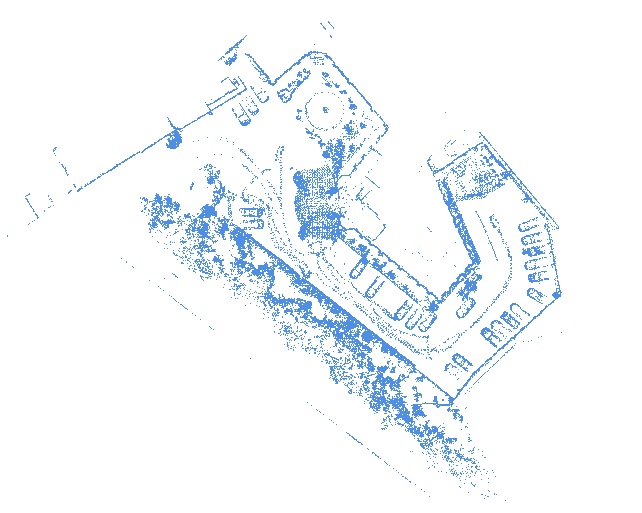
\includegraphics[width=0.6\textwidth]{resources/basic-point-cloud/bev.pdf}  
	\caption{Converting a point cloud to a bird's-eye view}  
	\label{fig:bev-example}  
\end{figure}  

Many path-planning algorithms, such as A* and D* \cite{Delling2009}, operate on grid maps, while perception or obstacle-avoidance algorithms can also use grid maps as input \cite{Sabe2004}. As seen, most obstacle information is preserved when converting point clouds to grid maps, though dynamic objects may leave smearing effects. We will discuss the probabilistic mechanism of grid maps in the 2D LiDAR SLAM chapter, which effectively mitigates the impact of dynamic objects.  

Some readers might wonder: If point clouds can be projected into a bird's-eye view, can they also be projected from other angles? While BEV is the most intuitive choice for top-down observation, similar logic can be applied to generate front or side views, which are computationally equivalent. However, another useful representation for algorithms is the \textbf{range image}.  

The concept of a range image aligns with that of RGB-D cameras. To ensure consistency between depth and color images, RGB-D cameras project point clouds into the color camera's frame. Similarly, can LiDAR point clouds be projected into a virtual camera? The answer is yes. However, since LiDAR point clouds cover a full 360-degree field of view, the resulting image is panoramic. Here, the horizontal axis represents the LiDAR's azimuth angle, while the vertical axis corresponds to the elevation angle. Alternatively, if the elevation angles for each scan line are known, the \textbf{line number} can serve as the vertical axis. Both methods produce what is known as a range image.  

As before, we provide an example to illustrate the appearance of a range image. While generating range images directly from raw LiDAR data (e.g., using block IDs or azimuth angles from packets) is more efficient, this approach depends on the specific LiDAR model. Our example uses post-processed point clouds, requiring only an additional azimuth angle calculation step.  

\begin{lstlisting}[language=c++,caption=src/ch5/scan\_to\_range\_image.cc]
DEFINE_string(pcd_path, "./data/ch5/scan_example.pcd", "Point cloud file path");
DEFINE_double(azimuth_resolution_deg, 0.3, "Azimuth resolution (degrees)");
DEFINE_int32(elevation_rows, 16, "Number of rows for elevation");
DEFINE_double(elevation_range, 15.0, "Elevation range");  // VLP-16 has ±15 degree range
DEFINE_double(lidar_height, 1.128, "LiDAR mounting height");

void GenerateRangeImage(PointCloudType::Ptr cloud) {
	int image_cols = int(360 / FLAGS_azimuth_resolution_deg);  // 360 degrees horizontally divided by resolution
	int image_rows = FLAGS_elevation_rows;                     // Fixed number of rows
	LOG(INFO) << "range image: " << image_rows << "x" << image_cols;
	
	// Create HSV image for better distance visualization
	cv::Mat image(image_rows, image_cols, CV_8UC3, cv::Scalar(0, 0, 0));
	
	double ele_resolution = FLAGS_elevation_range * 2 / FLAGS_elevation_rows;  // Elevation resolution
	
	for (const auto& pt : cloud->points) {
		double azimuth = atan2(pt.y, pt.x) * 180 / M_PI;
		double range = sqrt(pt.x * pt.x + pt.y * pt.y);
		double elevation = atan2((pt.z - FLAGS_lidar_height), range) * 180 / M_PI;
		
		// Normalize azimuth to 0~360
		if (azimuth < 0) {
			azimuth += 360;
		}
		
		int x = int(azimuth / FLAGS_azimuth_resolution_deg);                      // Column
		int y = int((elevation + FLAGS_elevation_range) / ele_resolution + 0.5);  // Row
		
		if (x >= 0 && x < image.cols && y >= 0 && y < image.rows) {
			image.at<cv::Vec3b>(y, x) = cv::Vec3b(uchar(range / 100 * 255.0), 255, 127);
		}
	}
	
	// Flip along Y-axis to make Z-up correspond to image-up
	cv::Mat image_flipped;
	cv::flip(image, image_flipped, 0);
	
	// Convert HSV to RGB
	cv::Mat image_rgb;
	cv::cvtColor(image_flipped, image_rgb, cv::COLOR_HSV2BGR);
	cv::imwrite("./range_image.png", image_rgb);
}
\end{lstlisting}

Several details require attention in this program, such as degree-radian conversion and image flipping along the Y-axis. We use HSV color space to display range information, making distance variations more visually apparent. To convert a single scan to a range image, run:

\begin{lstlisting}[language=sh,caption=Terminal input:]
bin/scan_to_range_image 
\end{lstlisting}

Readers can adjust parameters in gflags to achieve different conversion effects. The converted image is saved as range_image.png in the current directory. With default parameters, since the LiDAR has 16 scan lines, the output will be a long rectangular image of size 1200×16, as shown in Figure~\ref{fig:range-image-example}. The image height can be adjusted by changing the number of elevation rows. This representation resembles camera images but without perspective projection. Some algorithms discussed later will use range images to extract vertical features for localization. Readers can also try identifying ground regions and prominent pole-like objects in this image.

\begin{figure}[!htp]
	\centering
	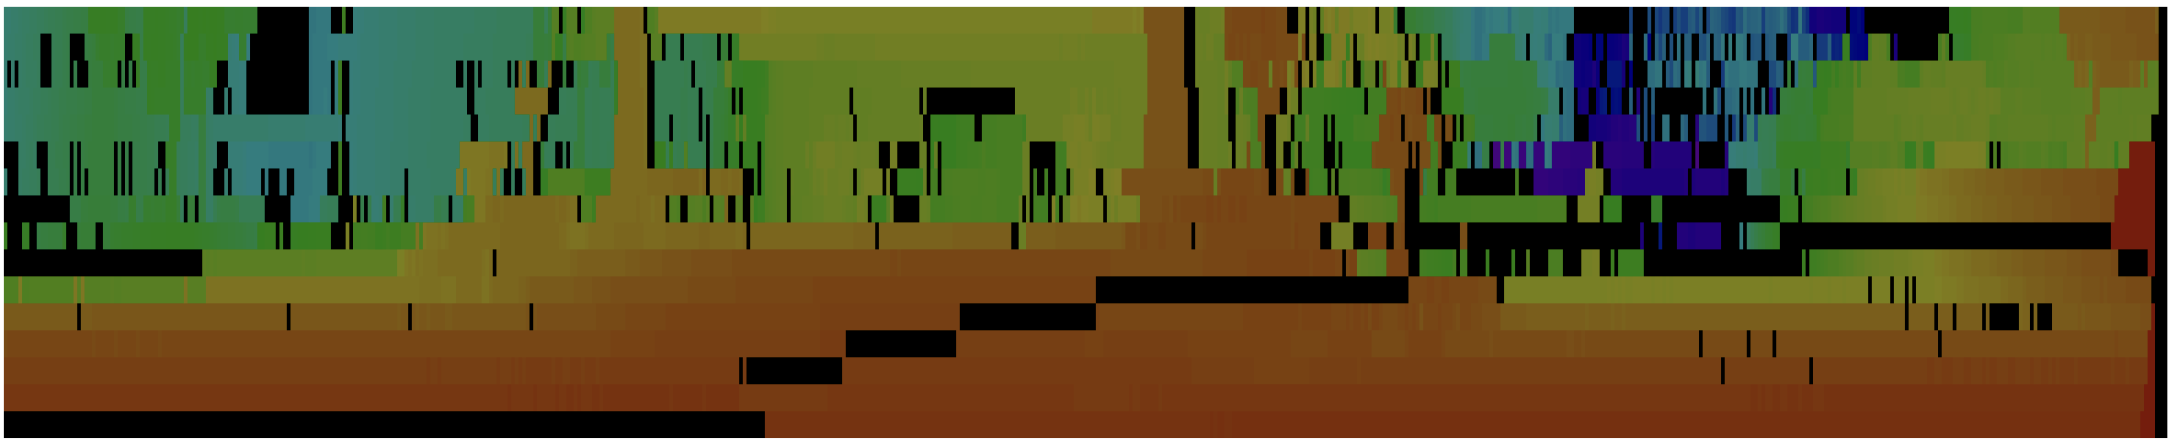
\includegraphics[width=0.8\textwidth]{resources/basic-point-cloud/range-image-raw.png}
	\caption{Converting point cloud to range image. The original range image is hard to display, so we scaled it here.}
	\label{fig:range-image-example}
\end{figure}

\subsection{Alternative Representations}
In addition to the methods previously discussed, some research has applied RGB-D 3D reconstruction techniques to LiDAR point clouds, aiming to achieve better reconstruction quality (and visual effects). For instance, works like \cite{Park2017, Park2018} employ Surfel maps to restore local surface reconstruction effects based on point clouds, while \cite{Roldao2019} demonstrates surface reconstruction using LiDAR data. However, in autonomous driving scenarios, LiDAR's primary functions remain localization and obstacle detection, and these algorithms have yet to become mainstream. We mention these approaches for reference, and interested readers may explore the cited papers.  

Of course, regardless of the representation method, the fundamental measurement data from the LiDAR remains unchanged—it neither becomes artificially denser nor more information-rich. So why use representations like range images or bird's-eye views? The key observation is that while these methods do not alter the raw measurements, they fundamentally change the \textbf{neighborhood relationships between points}. In raw point clouds, the adjacency between points is not explicitly encoded. In contrast, bird's-eye views and range images inherently encode pixel-to-pixel spatial relationships, enabling image-based processing.  

For example, a vertical pillar in 3D space is distributed along the $Z$-axis, but in a range image, it appears as a feature along the $Y$-axis, while in a bird's-eye view, it collapses to a single point. This shift in distribution affects the performance of clustering or feature extraction algorithms. Consequently, some algorithms prefer to extract features from range images or bird's-eye views first, then compute their corresponding 3D positions.

\section{Nearest Neighbor Problem}
The nearest neighbor problem is one of the most fundamental issues in point cloud processing and a step that will be repeatedly invoked in many matching algorithms. The problem can be described very simply: Given a point cloud $\mathcal{X} = \{ \bm{x}_1, \ldots, \bm{x}_n\}$ containing $n$ points, we ask, which point is closest to a given point $\bm{x}_m$? Further, what are the $k$ nearest points to it? Or which points lie within a fixed range $r$ of it? The former is called $k$-nearest neighbor search (kNN), while the latter is called range search.  

Although this problem appears simple, solving it is not trivial, and there are many different approaches. We are particularly concerned with the efficiency of solving the nearest neighbor problem because this algorithm is typically invoked thousands or even millions of times. A small increase in computation time per call can lead to significant efficiency differences in the overall matching algorithm. Below, we introduce nearest neighbor methods in order of increasing complexity, which also aligns with the historical development of algorithmic techniques.  

The algorithms in this chapter will emphasize parallelization, as point cloud algorithms require nearest neighbor searches on a large number of points, making parallel performance a critical consideration.  

\subsection{Brute-Force Nearest Neighbor Search}  
The brute-force nearest neighbor search (BF search) is the simplest and most intuitive method, requiring no auxiliary data structures\footnote{Sometimes referred to as linear search \cite{Weber1998}.} \cite{Kuang2009}. If we search for the nearest neighbor (NN) of a point, we call it \textbf{brute-force nearest neighbor search}; if we search for the $k$ nearest neighbors, we call it brute-force $k$-nearest neighbor search. Overall, this is a straightforward but computationally intensive approach.  

\begin{mdframed}
	\paragraph{Brute-Force Nearest Neighbor Search}  
	Given a point cloud $\mathcal{X}$ and a query point $\bm{x}_m$, compute the distance between $\bm{x}_m$ and every point in $\mathcal{X}$, then return the minimum distance.  
\end{mdframed}  

Similarly, the brute-force $k$-nearest neighbor search can be defined as:  

\begin{mdframed}
	\paragraph{Brute-Force $k$-Nearest Neighbor (BF kNN)}  
	\begin{enumerate}
		\item For a given point cloud $\mathcal{X}$ and query point $\bm{x}_m$, compute the distance between $\bm{x}_m$ and every point in $\mathcal{X}$.  
		\item Sort the results from step 1.  
		\item Select the $k$ nearest points.  
		\item Repeat steps 1–3 for all $\bm{x}_m$.  
	\end{enumerate}
\end{mdframed}  

Alternatively, we can maintain only the top $k$ results during computation, comparing each new distance with the existing ones to save storage space.  

It is clear that the brute-force method requires traversing the entire point cloud each time. For a point cloud of size $n$, its complexity is $O(n)$. When dealing with the matching problem between two point clouds (assuming both have $n$ points), the complexity of brute-force nearest neighbor search becomes $O(n^2)$. This is obviously a time-consuming method, and BF kNN also requires an additional sorting step. However, the computation for each point in BF search is very simple and does not rely on complex data structures, making it highly parallelizable. A GPU-accelerated BF search or BF kNN may outperform some more sophisticated algorithms \cite{Garcia2008, Li2015}. In most engineering applications, it is also unnecessary to search the entire target point cloud $\mathcal{X}$—instead, searches can be restricted to a predefined local region. Therefore, BF search remains highly practical in many real-world applications.  

To facilitate comparison, we will use a pair of example point clouds (see \texttt{data/ch5/first.pcd} and \texttt{second.pcd}) as data sources in this section, applying various methods to compute their nearest neighbors. Considering that readers may not have access to GPUs, we provide both single-threaded and multi-threaded CPU implementations of nearest neighbor search. Subsequent algorithms will also compare the efficiency of single-threaded versus multi-threaded implementations. For simpler methods (such as the BF method in this section), we will also compare handwritten implementations with those provided by the PCL library.

\subsubsection{Brute-Force Nearest Neighbor Implementation}
The BF (Brute-Force) matching implementation is straightforward. Using C++17's parallel mechanisms, it's easy to extend the single-threaded version to a multi-threaded one. We utilize STL algorithms to implement both single-threaded and multi-threaded BF matching, first defining a brute-force nearest neighbor search for a single point and then extending it to compute nearest neighbors for multiple points.

\begin{lstlisting}[language=c++, caption=src/ch5/bfnn.cc]
int bfnn_point(CloudPtr cloud, const Vec3f& point) {
	return std::min_element(cloud->points.begin(), cloud->points.end(),
	[&point](const PointType& pt1, const PointType& pt2) -> bool {
		return (pt1.getVector3fMap() - point).squaredNorm() <
		(pt2.getVector3fMap() - point).squaredNorm();
	}) - cloud->points.begin();
}

void bfnn_cloud_mt(CloudPtr cloud1, CloudPtr cloud2, std::vector<std::pair<size_t, size_t>>& 
matches) {
	// Generate indices first
	std::vector<size_t> index(cloud1->size());
	std::for_each(index.begin(), index.end(), [idx = 0](size_t& i) mutable { i = idx++; });
	
	// Parallel for_each
	matches.resize(index.size());
	std::for_each(std::execution::par_unseq, index.begin(), index.end(), [&](auto idx) {
		matches[idx].second = idx;
		matches[idx].first = bfnn_point(cloud1, ToVec3f(cloud2->points[idx]));
	});
}
\end{lstlisting}

In the single-point nearest neighbor search, we take a point as input, compute the distance to every point in the cloud, and then retrieve the minimum. This is achieved using `std::min_element` and a lambda function. The parallel version uses `std::execution` to concurrently invoke the single-point nearest neighbor algorithm for each point.

Next, let's examine the test program. This section uses gtest to benchmark various nearest neighbor methods for comparison:

\begin{lstlisting}[language=c++,caption=src/ch5/test\_nn.cc]
TEST(CH5_TEST, BFNN) {
	sad::CloudPtr first(new sad::PointCloudType), second(new sad::PointCloudType);
	pcl::io::loadPCDFile(FLAGS_first_scan_path, *first);
	pcl::io::loadPCDFile(FLAGS_second_scan_path, *second);
	
	if (first->empty() || second->empty()) {
		LOG(ERROR) << "cannot load cloud";
		FAIL();
	}
	
	// Apply voxel grid downsampling to 0.05
	sad::VoxelGrid(first);
	sad::VoxelGrid(second);
	
	// Benchmark single-threaded and multi-threaded brute-force matching
	sad::evaluate_and_call(
	[&first, &second]() {
		std::vector<std::pair<size_t, size_t>> matches;
		sad::bfnn_cloud(first, second, matches);
	},
	"Brute-Force Matching (Single-threaded)", 5);
	sad::evaluate_and_call(
	[&first, &second]() {
		std::vector<std::pair<size_t, size_t>> matches;
		sad::bfnn_cloud_mt(first, second, matches);
	},
	"Brute-Force Matching (Multi-threaded)", 5);
	
	SUCCEED();
}
\end{lstlisting}

Here, the `evaluate_and_call` function is used. This function invokes a specified method a fixed number of times and measures its execution time:
\begin{lstlisting}[language=c++,caption=src/common/sys\_utils.h]
/**
* Measure code execution time
* @tparam FuncT
* @param func  Function to be called
* @param func_name  Function name
* @param times  Number of calls
*/
template <typename FuncT>
void evaluate_and_call(FuncT func, const std::string &func_name = "", int times = 10) {
	double total_time = 0;
	for (int i = 0; i < times; ++i) {
		auto t1 = std::chrono::high_resolution_clock::now();
		func();
		auto t2 = std::chrono::high_resolution_clock::now();
		total_time += std::chrono::duration_cast<std::chrono::duration<double>>(t2 - t1).count() * 1000;
	}
	
	LOG(INFO) << "Method " << func_name << " average call time/iterations: " << total_time / times << "/" << times << " ms.";
}
\end{lstlisting}

We call both the single-threaded and multi-threaded versions five times each and compute their average execution times.

\begin{lstlisting}[language=sh,caption=Terminal output]
bin/test_nn --gtest_filter=CH5_TEST.BFNN 
Note: Google Test filter = CH5_TEST.BFNN
[==========] Running 1 test from 1 test suite.
[----------] Global test environment set-up.
[----------] 1 test from CH5_TEST
[ RUN      ] CH5_TEST.BFNN
Failed to find match for field 'intensity'.
Failed to find match for field 'intensity'.
I0116 13:40:57.001132 267085 test_nn.cc:36] points: 18869, 18779
I0116 13:41:04.886138 267085 sys_utils.h:32] Method Brute-Force Matching (Single-threaded) average call time/iterations: 1576.98/5 ms.
I0116 13:41:05.291601 267085 sys_utils.h:32] Method Brute-Force Matching (Multi-threaded) average call time/iterations: 81.0873/5 ms.
\end{lstlisting}

As shown, for point clouds with around 18,000 points, the single-threaded brute-force matching takes approximately 1.5 seconds, while the multi-threaded version requires only 81 milliseconds. These benchmarks are highly dependent on machine performance. The tests were conducted on an i9-12900KF machine, and readers may observe different results (possibly significant variations) on their own systems. However, the relative speed differences between algorithms remain consistent for evaluation purposes. 

The advantage of brute-force matching is that it computes matches for every pair of points, ensuring correctness. Subsequent methods may not guarantee this. We now use brute-force matching results as a benchmark to evaluate the performance of other approaches.

\subsection{Grid and Voxel Methods}
Brute-force search (or linear search) essentially involves traversing and searching through a data structure. Students familiar with data structures would immediately suggest that for sorted containers, binary search is clearly faster than sequential search. With a bit more recall, one might remember that binary search reduces the complexity to \(O(\log_2 N)\) compared to linear search. This line of thinking leads to the binary trees and K-d trees discussed in Section~\ref{sec:binary-tree}. Tree structures index the data itself. On the other hand, since point clouds are spatial data, we can also index them spatially. Depending on the indexing method, this leads to 2D grid or 3D voxel approaches, and further to quadtrees and octrees. This section focuses on the latter category.

\begin{figure}[!htp]
	\centering
	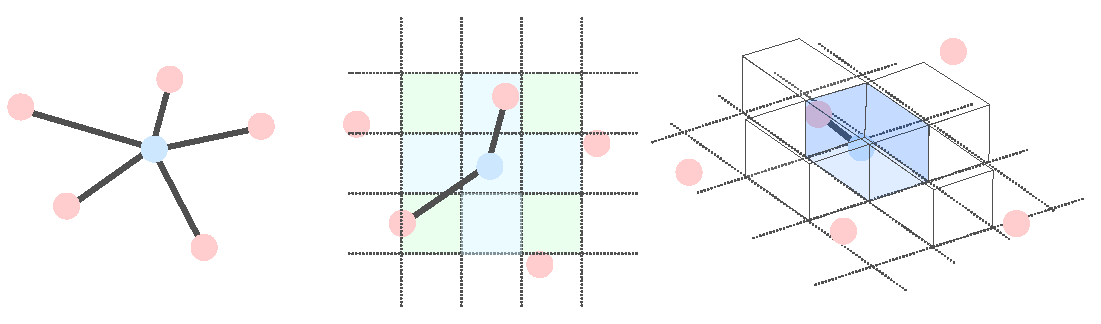
\includegraphics[width=0.8\textwidth]{resources/basic-point-cloud/grid-and-voxel.pdf}
	\caption{Nearest neighbor search: grid and voxel methods. In the grid method, space is divided into 2D projected grids, and the nearest points are searched within the surrounding grids of the query point. In voxel-based methods, space is divided into 3D voxels, and the search is performed in adjacent voxels. For simplicity, only four surrounding voxels are shown here; in practice, the top and bottom voxels should also be included, totaling six.}
	\label{fig:grid-and-voxel}
\end{figure}

\subsubsection{Grid-Based Nearest Neighbor Search}
If we partition the point cloud spatially into grids, we can compute the grid position for each point and index all points spatially, as shown in Figure~\ref{fig:grid-and-voxel}. When searching for the nearest neighbor, we first compute the grid cell containing the query point and then search for its nearest neighbor in the surrounding grid cells. The nearest neighbor in the grid can be easily defined, such as the adjacent cells above, below, left, and right, significantly narrowing the search scope. However, there are a few considerations when generating the grid:

\begin{itemize}
	\item Based on the density of the point cloud, we need to predefine the \textbf{resolution} of the grid, which is a \textbf{hyperparameter}—a parameter related to the computational task. If the grid cells are too large, each cell will contain many points, reducing the efficiency of nearest neighbor search. If the cells are too small, the number of cells increases, and due to the sparsity of the point cloud, the nearest neighbor might not lie in the adjacent cells, potentially missing the true nearest neighbor. This method is highly sensitive to \textbf{hyperparameters} and requires empirical tuning.
	\item Since grid boundaries are discrete, when searching for the nearest neighbor, we should not only search within the current grid cell but also in its \textbf{surrounding} cells. The definition of \textbf{surrounding} can vary. For 2D grids, we might consider the four adjacent cells (up, down, left, right) as "surrounding," or include the four corners for a total of eight cells. Clearly, the more surrounding cells included, the more cells need to be searched, reducing algorithmic efficiency. Thus, a reasonable value must be chosen in practice. This issue also applies to voxel methods, where we can similarly define six adjacent voxels or include the eight corners for a total of 14 neighboring voxels.
	\item Due to the limited scope of grid searches, it is possible to fail to find the nearest neighbor for a given point. This is quite different from brute-force search, which can match all points and thus guarantees finding the nearest neighbor for every point. Grid methods, however, do not always guarantee this. Therefore, in addition to evaluating the computational efficiency of grid methods, their \textbf{correctness} must also be assessed. The same applies to subsequent algorithms.
\end{itemize}

\subsubsection{Voxel-Based Nearest Neighbor Search}
Voxel-based nearest neighbor search is very similar to the grid method. While the grid method partitions space into 2D grids, the voxel method divides space into 3D \textbf{voxels}—think of them as small cubes forming a partitioning scheme. A voxel is directly adjacent to six surrounding voxels; including diagonals adds another eight, for a total of 14 adjacent voxels.

\subsubsection{Implementation}
Since 2D grids and voxel methods are very similar, we implement them using a template class. We use the dimensionality as a template parameter and employ 2D or 3D integer vectors as grid indices to unify the implementation of 2D and 3D grids, keeping the code as compact as possible. Additionally, we define neighboring relationships through enumerations, allowing users to specify the desired adjacency type.

First, let's look at the basic definition of grid-based nearest neighbor search:
\begin{lstlisting}[language=c++,caption=src/ch5/gridnn.hpp]
/**
* Grid-based nearest neighbor search
* @tparam dim Template parameter, using 2D or 3D voxels
*/
template <int dim>
class GridNN {
	public:
	using KeyType = Eigen::Matrix<int, dim, 1>;
	using PtType = Eigen::Matrix<float, dim, 1>;
	
	enum class NearbyType {
		CENTER,  // Only consider the center
		// For 2D
		NEARBY4,  // Up, down, left, right
		NEARBY8,  // Up, down, left, right + four corners
		
		// For 3D
		NEARBY6,  // Up, down, left, right, front, back
	};
	
	private:
	float resolution_ = 0.1;       // Resolution
	float inv_resolution_ = 10.0;  // Inverse of resolution
	
	NearbyType nearby_type_ = NearbyType::NEARBY4;
	std::unordered_map<KeyType, std::vector<size_t>, hash_vec<dim>> grids_;  // Grid data
	CloudPtr cloud_;
	
	std::vector<KeyType> nearby_grids_;  // Nearby grids
};
\end{lstlisting}

We define neighboring relationships as the enumeration type `NearbyType`, and the actual grid data is stored in an `std::unordered_map` (hash table). Since point clouds are sparse, the corresponding grids are also sparse, so empty grids need not be retained where no data exists. Hash tables are highly effective in this application scenario. We define the key of this table as a 2D or 3D integer vector and implement the hash function as follows:

\begin{lstlisting}[language=c++,caption=src/common/eigen\_types.h]
/// Vector hash
template <int N>
struct hash_vec {
	inline size_t operator()(const Eigen::Matrix<int, N, 1>& v) const;
};

template <>
inline size_t hash_vec<2>::operator()(const Eigen::Matrix<int, 2, 1>& v) const {
	return size_t(((v[0] * 73856093) ^ (v[1] * 471943)) % 10000000);
}

template <>
inline size_t hash_vec<3>::operator()(const Eigen::Matrix<int, 3, 1>& v) const {
	return size_t((v[0] * 73856093) ^ (v[1] * 471943) ^ (v[2] * 83492791) % 10000000);
}
\end{lstlisting}

The `hash_vec` function is a template function with two specializations for 2D and 3D spatial hash functions, respectively. According to the literature \cite{Teschner2003}, spatial hash functions can be implemented by multiplying each dimension's data by a large prime number, then taking the XOR, and finally applying modulo with a large integer. For a spatial point \(\bm{p}=[p_x, p_y, p_z]\), using three large prime numbers \(n_1, n_2, n_3\) and a large integer \(N\), its hash function can be defined as:
\begin{equation}\label{key}
	\text{hash}(\bm{p}) = ((p_x n_1) ~ \mathrm{xor}~ (p_y n_2) ~\mathrm{xor}~ (p_z n_3))~\text{mod}~ N.
\end{equation}

Similarly, we can define a hash function for 2D spatial points. Combined with the template parameter `dim` of the `GridNN` class, these can be used as implementations for the hash function in `std::unordered_map`. Then, we define their nearest neighbors in the `nearby_grids_` member variable:

\begin{lstlisting}[language=c++,caption=src/ch5/gridnn.hpp]
template <>
void GridNN<2>::GenerateNearbyGrids() {
	if (nearby_type_ == NearbyType::CENTER) {
		nearby_grids_.emplace_back(KeyType::Zero());
	} else if (nearby_type_ == NearbyType::NEARBY4) {
		nearby_grids_ = {Vec2i(0, 0), Vec2i(-1, 0), Vec2i(1, 0), Vec2i(0, 1), Vec2i(0, -1)};
	} else if (nearby_type_ == NearbyType::NEARBY8) {
		nearby_grids_ = {
			Vec2i(0, 0),   Vec2i(-1, 0), Vec2i(1, 0),  Vec2i(0, 1), Vec2i(0, -1),
			Vec2i(-1, -1), Vec2i(-1, 1), Vec2i(1, -1), Vec2i(1, 1),
		};
	}
}

template <>
void GridNN<3>::GenerateNearbyGrids() {
	if (nearby_type_ == NearbyType::CENTER) {
		nearby_grids_.emplace_back(KeyType::Zero());
	} else if (nearby_type_ == NearbyType::NEARBY6) {
		nearby_grids_ = {KeyType(0, 0, 0),  KeyType(-1, 0, 0), KeyType(1, 0, 0), KeyType(0, 1, 0),
			KeyType(0, -1, 0), KeyType(0, 0, -1), KeyType(0, 0, 1)};
	}
}
\end{lstlisting}

Using specialized template classes, we can define different neighbor generation methods for 2D and 3D voxels. The 2D grid allows selecting 0, 4, or 8 nearest neighbors, while the 3D voxel allows selecting 0 or 6 nearest neighbors (the 14-neighbor case is left as an exercise for the reader). Now, let's implement the nearest neighbor search logic:
\begin{enumerate}
	\item First, compute the grid cell containing the given point.
	\item Based on the nearest neighbor definition, search the nearby grid cells.
	\item Collect the results from step 2 and use brute-force matching to compute the nearest neighbor within these grid cells.
\end{enumerate}

Step 3 can reuse the brute-force matching code from earlier. This process is the same for both 2D and 3D grids, so we use the same interface at the code level. The single nearest neighbor search function is as follows:

\begin{lstlisting}[language=c++,caption=src/ch5/gridnn.hpp]
template <int dim>
bool GridNN<dim>::GetClosestPoint(const PointType& pt, PointType& closest_pt, size_t& idx) {
	// Search for the nearest neighbor in the grid cells around pt
	std::vector<size_t> idx_to_check;
	auto key = Pos2Grid(ToEigen<float, dim>(pt));
	
	std::for_each(nearby_grids_.begin(), nearby_grids_.end(), [&key, &idx_to_check, this](const KeyType& delta) {
		auto dkey = key + delta;
		auto iter = grids_.find(dkey);
		if (iter != grids_.end()) {
			idx_to_check.insert(idx_to_check.end(), iter->second.begin(), iter->second.end());
		}
	});
	
	if (idx_to_check.empty()) {
		return false;
	}
	
	// Brute-force NN in cloud_[idx]
	idx = bfnn_point(cloud_, idx_to_check, ToVec3f(pt));
	closest_pt = cloud_->points[idx];
	return true;
}

template <int dim>
Eigen::Matrix<int, dim, 1> GridNN<dim>::Pos2Grid(const Eigen::Matrix<float, dim, 1>& pt) {
	return (pt * inv_resolution_).template cast<int>();
}
\end{lstlisting}

The point cloud version simply adds a concurrent wrapper around this function:
\begin{lstlisting}[language=c++,caption=src/ch5/gridnn.hpp]
template <int dim>
bool GridNN<dim>::GetClosestPointForCloudMT(CloudPtr ref, CloudPtr query,
std::vector<std::pair<size_t, size_t>>& matches) {
	// Essentially the same as the serial version, but matches must be preallocated, with invalid matches filled on failure
	std::vector<size_t> index(query->size());
	std::for_each(index.begin(), index.end(), [idx = 0](size_t& i) mutable { i = idx++; });
	matches.resize(index.size());
	
	std::for_each(std::execution::par_unseq, index.begin(), index.end(), [this, &matches, &query](const size_t& idx) {
		PointType cp;
		size_t cp_idx;
		if (GetClosestPoint(query->points[idx], cp, cp_idx)) {
			matches[idx] = {cp_idx, idx};
		} else {
			matches[idx] = {math::kINVALID_ID, math::kINVALID_ID};
		}
	});
	
	return true;
}
\end{lstlisting}


Now let's test the performance of various 2D and 3D voxel methods under different nearest neighbor definitions. Note that in addition to testing performance, we should also focus on whether these nearest neighbors are correct. In fact, grid-based nearest neighbor search may encounter two types of errors:

\begin{enumerate}
	\item The nearest neighbor detected by the grid method is not actually the nearest neighbor in reality. This is called a \textbf{false positive} (FP). The number of false positives in an experiment is denoted as \(FP\).
	\item A true nearest neighbor in reality is not detected by the grid method. This is called a \textbf{false negative} (FN). The number of false negatives in an experiment is denoted as \(FN\).
\end{enumerate}

Using the definitions of \(FP\) and \(FN\), we can define the algorithm's \textbf{precision} and \textbf{recall}. Let \(m\) be the total number of nearest neighbors computed by the algorithm and \(n\) be the total number of ground truth nearest neighbors. Then, precision and recall are defined as:
\begin{equation}\label{key}
	\text{precision} = \frac{1-FP}{m}, \quad \text{recall} = \frac{1-FN}{n}
\end{equation}

Precision describes the correctness of the nearest neighbors detected by the algorithm, while recall describes the proportion of true results that the algorithm successfully detects. A well-performing algorithm should achieve high values in both metrics, but this may come at the cost of slower performance. For example, brute-force matching can achieve 100\% precision and recall, but its computational time is often unacceptable.

When testing nearest neighbor algorithms, we can evaluate their precision and recall using the following method:
\begin{lstlisting}[language=c++,caption=src/ch5/test\_nn.cc]
/**
* Evaluate the correctness of nearest neighbor matches
* @param truth Ground truth matches
* @param esti  Estimated matches
*/
void EvaluateMatches(const std::vector<std::pair<size_t, size_t>>& truth,
const std::vector<std::pair<size_t, size_t>>& esti) {
	int fp = 0;  // false-positive: exists in esti but not in truth
	int fn = 0;  // false-negative: exists in truth but not in esti
	
	/// Check if a match exists in another container
	auto exist = [](const std::pair<size_t, size_t>& data, const std::vector<std::pair<size_t, size_t>>& vec) -> bool {
		return std::find(vec.begin(), vec.end(), data) != vec.end();
	};
	
	for (const auto& d : esti) {
		if (!exist(d, truth)) {
			fp++;
		}
	}
	
	for (const auto& d : truth) {
		if (!exist(d, esti)) {
			fn++;
		}
	}
	
	float precision = 1.0 - float(fp) / esti.size();
	float recall = 1.0 - float(fn) / truth.size();
	LOG(INFO) << "precision: " << precision << ", recall: " << recall << ", fp: " << fp << ", fn: " << fn;
}
\end{lstlisting}

Next, we test the grid-based nearest neighbor method:

\begin{lstlisting}[language=c++,caption=src/ch5/test\_nn.cc]
TEST(CH5_TEST, GRID_NN) {
	// Code for loading point clouds omitted
	std::vector<std::pair<size_t, size_t>> truth_matches;
	sad::bfnn_cloud(first, second, truth_matches);
	
	// Compare different types of grids
	sad::GridNN<2> grid0(0.1, sad::GridNN<2>::NearbyType::CENTER), grid4(0.1, sad::GridNN<2>::NearbyType::NEARBY4),
	grid8(0.1, sad::GridNN<2>::NearbyType::NEARBY8);
	sad::GridNN<3> grid3(0.1, sad::GridNN<3>::NearbyType::NEARBY6);
	
	grid0.SetPointCloud(first);
	grid4.SetPointCloud(first);
	grid8.SetPointCloud(first);
	grid3.SetPointCloud(first);
	
	// Evaluate various versions of Grid NN
	
	LOG(INFO) << "===================";
	std::vector<std::pair<size_t, size_t>> matches;
	sad::evaluate_and_call(
	[&first, &second, &grid0, &matches]() { grid0.GetClosestPointForCloud(first, second, matches); },
	"Grid0 Single-threaded", 10);
	EvaluateMatches(truth_matches, matches);
	
	LOG(INFO) << "===================";
	sad::evaluate_and_call(
	[&first, &second, &grid0, &matches]() { grid0.GetClosestPointForCloudMT(first, second, matches); },
	"Grid0 Multi-threaded", 10);
	EvaluateMatches(truth_matches, matches);
	
	/// Other test methods are similar and omitted
}
\end{lstlisting}

We primarily compare the runtime and nearest neighbor performance of each method. Readers should observe the same precision and recall metrics, though runtime may vary.

\begin{lstlisting}[language=sh,caption=Terminal output:]
./bin/test_nn --gtest_filter=CH5_TEST.GRID_NN 
I0116 17:04:58.055471 276361 test_nn.cc:125] ===================
I0116 17:04:58.065711 276361 sys_utils.h:32] Method Grid0 Single-threaded average call time/iterations: 1.02376/10 ms.
I0116 17:04:58.065724 276361 test_nn.cc:65] truth: 18869, esti: 8518
I0116 17:04:58.099488 276361 test_nn.cc:91] precision: 0.486382, recall: 0.219566, fp: 4375, fn: 14726
I0116 17:04:58.099493 276361 test_nn.cc:132] ===================
I0116 17:04:58.104143 276361 sys_utils.h:32] Method Grid0 Multi-threaded average call time/iterations: 0.464818/10 ms.
I0116 17:04:58.104161 276361 test_nn.cc:65] truth: 18869, esti: 18779
I0116 17:04:58.158778 276361 test_nn.cc:91] precision: 0.486382, recall: 0.219566, fp: 4375, fn: 14726
I0116 17:04:58.158783 276361 test_nn.cc:138] ===================
I0116 17:04:58.202162 276361 sys_utils.h:32] Method Grid4 Single-threaded average call time/iterations: 4.33758/10 ms.
I0116 17:04:58.202165 276361 test_nn.cc:65] truth: 18869, esti: 13272
I0116 17:04:58.246877 276361 test_nn.cc:91] precision: 0.646775, recall: 0.454926, fp: 4688, fn: 10285
I0116 17:04:58.246881 276361 test_nn.cc:144] ===================
I0116 17:04:58.254035 276361 sys_utils.h:32] Method Grid4 Multi-threaded average call time/iterations: 0.715278/10 ms.
I0116 17:04:58.254041 276361 test_nn.cc:65] truth: 18869, esti: 18779
I0116 17:04:58.308115 276361 test_nn.cc:91] precision: 0.646775, recall: 0.454926, fp: 4688, fn: 10285
I0116 17:04:58.308118 276361 test_nn.cc:150] ===================
I0116 17:04:58.379315 276361 sys_utils.h:32] Method Grid8 Single-threaded average call time/iterations: 7.11945/10 ms.
I0116 17:04:58.379319 276361 test_nn.cc:65] truth: 18869, esti: 14613
I0116 17:04:58.425294 276361 test_nn.cc:91] precision: 0.728735, recall: 0.564365, fp: 3964, fn: 8220
I0116 17:04:58.425297 276361 test_nn.cc:156] ===================
I0116 17:04:58.433573 276361 sys_utils.h:32] Method Grid8 Multi-threaded average call time/iterations: 0.827275/10 ms.
I0116 17:04:58.433579 276361 test_nn.cc:65] truth: 18869, esti: 18779
I0116 17:04:58.485752 276361 test_nn.cc:91] precision: 0.728735, recall: 0.564365, fp: 3964, fn: 8220
I0116 17:04:58.485755 276361 test_nn.cc:162] ===================
I0116 17:04:58.513800 276361 sys_utils.h:32] Method Grid 3D Single-threaded average call time/iterations: 2.80424/10 ms.
I0116 17:04:58.513803 276361 test_nn.cc:65] truth: 18869, esti: 8572
I0116 17:04:58.540259 276361 test_nn.cc:91] precision: 0.911339, recall: 0.414012, fp: 760, fn: 11057
I0116 17:04:58.540262 276361 test_nn.cc:168] ===================
I0116 17:04:58.545367 276361 sys_utils.h:32] Method Grid 3D Multi-threaded average call time/iterations: 0.510082/10 ms.
I0116 17:04:58.545372 276361 test_nn.cc:65] truth: 18869, esti: 18779
I0116 17:04:58.589224 276361 test_nn.cc:91] precision: 0.911339, recall: 0.414012, fp: 760, fn: 11057
\end{lstlisting}

From the results, we can see that for grid-based methods, increasing the number of neighboring grids increases runtime, while the multi-threaded version significantly outperforms the single-threaded version. The voxel method performs similarly to the grid method in terms of efficiency\footnote{This is because we used \texttt{std::unordered\_map} to index grid keys. If \texttt{std::map} were used, a noticeable efficiency difference would emerge—readers are encouraged to try this.}, and the multi-threaded version is also significantly better than the single-threaded version. For many real-time applications, nearest neighbor query times below 1 millisecond are acceptable.

In terms of precision and recall, 3D voxels significantly outperform 2D grids, and 2D grids show notable improvements as the number of neighbors increases. The grid resolution also affects performance. This test used a grid resolution of 0.1, which is typically too small for autonomous driving datasets. Increasing it to around 0.5 would significantly improve precision and recall but at the cost of performance. Readers are encouraged to experiment with different grid sizes to observe performance under various parameters. Note that this test evaluates single nearest neighbor cases; \(k\)-nearest neighbor metrics are generally harder to achieve.

Figure~\ref{fig:grid-bad-cases} illustrates the false negative and false positive issues inherent in grid-based nearest neighbor search. Since grids fundamentally impose rigid spatial partitioning, problems arise when a point lies near partition boundaries. In the left portion of the figure, the red point should be the true nearest neighbor of the blue point, but because it falls outside the neighboring grid cells being searched, the algorithm fails to detect it. Conversely, in the right portion, while the left red point has a greater Euclidean distance than the right red point, it gets incorrectly identified as the nearest neighbor simply because it's the only candidate within the searched neighboring grids. 

Expanding the neighborhood search range may mitigate these issues probabilistically. However, even with expanded ranges, partition boundaries persist, meaning false negatives and false positives will inevitably remain at these transitional zones.

\begin{figure}[!htp]
	\centering
	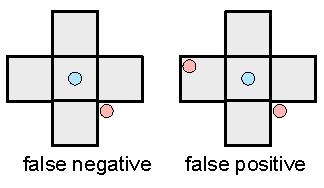
\includegraphics[width=0.4\textwidth]{resources/basic-point-cloud/grid-bad-cases.pdf}
	\caption{Schematic illustration of false positive/negative issues in grid-based nearest neighbor search}
	\label{fig:grid-bad-cases}
\end{figure}

This naturally leads to the question: Could we abandon fixed-distance partitioning in favor of more intelligent spatial subdivision methods? This is precisely the rationale behind K-d trees. However, compared to the tree-based data structures we'll discuss later, grid and voxel methods achieve respectable performance using simpler data structures while being inherently parallelizable. Together with tree structures, voxel-based approaches form the foundation of most modern matching algorithms and SLAM systems \cite{Koide2019,Koide2020,Huang2021a,Bai2022}. 

The key trade-off emerges: While tree structures provide more adaptive spatial partitioning that better handles boundary cases, their increased algorithmic complexity often offsets their theoretical advantages in practical implementations where parallel processing and memory locality significantly impact real-world performance. This explains why many state-of-the-art systems employ hybrid approaches, combining the brute-force efficiency of voxel methods with the adaptive precision of tree structures where needed.

Notably, the precision/recall metrics shown in our earlier benchmarks (0.91 precision for 3D voxels vs 0.73 for 2D 8-neighbor grids) demonstrate that dimensionality plays a crucial role - the additional spatial information in 3D inherently provides better disambiguation between true and false neighbors, even using similar search methodologies. This dimensional advantage becomes particularly important in applications like autonomous driving where the vertical dimension often provides critical discriminative information.

\subsection{Binary Trees and K-d Trees}
\label{sec:binary-tree}
Let us now return to the earlier idea: searching in a sorted container can significantly save time. Following this line of thought, we can propose data structures similar to binary search, such as Binary Search Trees (BST) and their high-dimensional counterpart: K-dimensional trees (K-d trees). Since point clouds belong to three-dimensional space, we will focus on introducing K-d trees.  

From data structure knowledge, searching in a sorted container using binary search is more efficient than linear search: binary search has a complexity of \(O(\log_2 N)\), while linear search is \(O(N)\). The binary search process itself is tree-like: for a given element \(x\) and container \(V\), we first compare \(x\) with the central element of the container. If \(x\) is smaller, we continue comparing it with the left half of the container; otherwise, we compare it with the right half. Based on this relationship, we can reorganize the container using a tree data structure to facilitate faster searches.  

This process does not require predefined partitioning thresholds. Additionally, binary trees have a space complexity of \(O(N)\) and a time complexity of \(O(\log_2 N)\), making them an ideal search method. The only drawback is that this approach is only effective for one-dimensional data. For high-dimensional data, points may be well-separated in one dimension but overlap in another, making binary trees and binary search unsuitable for direct application.  

The K-d tree \cite{Bentley1975}, originally proposed by Bentley Jon Louis, is a high-dimensional extension of binary trees, as illustrated in Figure~\ref{fig:kdtree}. A K-d tree is also a type of binary tree, where each node consists of left and right branches. In binary trees, we can use a single dimension to distinguish between left and right branches. However, in K-d trees, since we need to partition high-dimensional data, we use \textbf{hyperplanes} to separate the left and right branches (though for 3D points, the hyperplane is simply an ordinary 2D plane).  

There are methodological differences in \textbf{how to partition} the data. Theoretically, finding a hyperplane to separate two high-dimensional point sets can be viewed as a support vector machine (SVM) classification problem \cite{Cortes1995}. However, for K-d trees in SLAM, where both construction and search processes need to run in real-time, we typically choose simpler partitioning methods. The simplest is the \textbf{axis-aligned splitting plane}. Despite its intimidating name, it simply involves splitting the point cloud along any one of the axes, making it very easy to implement.  

\begin{figure}[!htp]
	\centering
	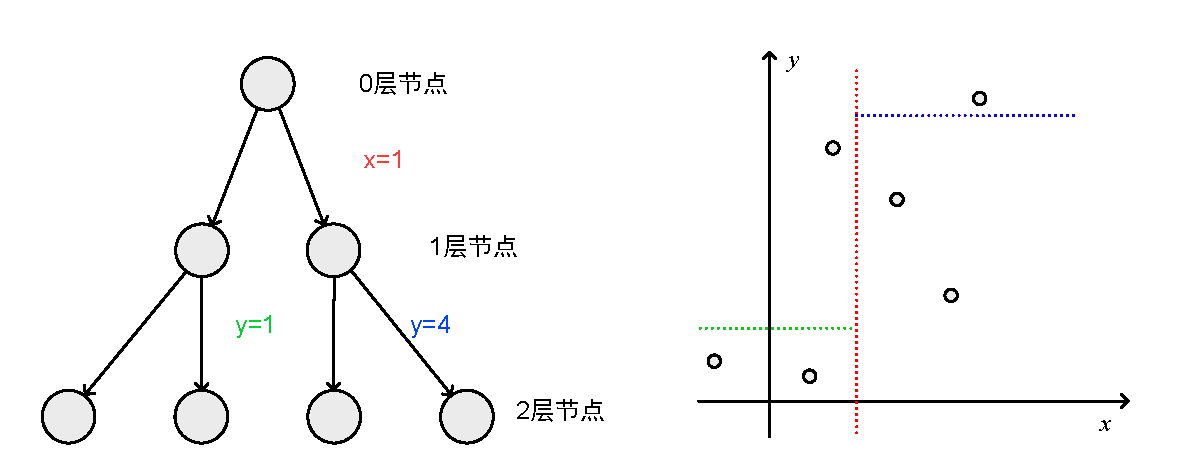
\includegraphics[width=0.8\textwidth]{resources/basic-point-cloud/kdtree.pdf}
	\caption{Schematic of a K-d tree. The left side shows the tree structure in the program, while the right side illustrates the partitioning relationships of each node.}
	\label{fig:kdtree}
\end{figure}

We can construct a K-d tree for a point cloud of any dimensionality, referred to as the \textbf{building process} or \textbf{tree construction}. Subsequently, we can perform kNN searches for any point in space, referred to as the \textbf{search process}. Depending on the search method, K-d trees can be categorized into \textbf{range search} (Search by range) and \textbf{K-nearest neighbor search} (Search by K nearest neighbors), with minor differences in their implementations.  

In a K-d tree, we use a tree structure to represent the spatial relationships of the point cloud, with the following rules:  
1. Each node has left and right branches.  
2. Leaf nodes represent points in the original point cloud. In practice, we can store point indices instead of the points themselves to save space.  
3. Non-leaf nodes store a splitting axis and a splitting threshold to define how the left and right branches are partitioned. For example, \(x = 1\) can be stored as splitting along the first axis with a threshold of 1. We define the left branch as taking values less than the threshold and the right branch as taking values greater than the threshold.  

With these conventions, we can implement the construction and search algorithms for K-d trees. Below, we briefly describe the algorithmic steps and then provide implementations and discussions of the results. Since K-d trees are fundamentally tree structures, most algorithms can be concisely implemented using recursion.

\subsection{Construction of K-d Trees}
In the construction process of a K-d tree, we primarily consider how to partition a given point cloud. Different partitioning strategies exist depending on the method used. Traditional approaches either alternate coordinate axes in a fixed order \cite{DeBerg1997} or calculate the dispersion of the current point cloud along each axis and select the axis with the highest dispersion as the splitting axis. Here, we focus on the latter method. Additionally, there are various variants such as implicit K-d trees \cite{Gros2007}, min-max K-d trees \cite{Duvenhage2009}, and relaxed K-d trees \cite{Duch1998}, which employ different strategies to handle partitioning or leaf node storage. For now, we will focus on the basic K-d tree.

\begin{mdframed}
	\textbf{Construction of a K-d Tree:}
	\begin{enumerate}
		\item \textbf{Input:} Point cloud data \(\bm{X} = \{\bm{x}_1, \ldots, \bm{x}_n\}\), where \(\bm{x}_i \in \mathbb{R}^{k}\).
		\item Consider inserting subset \(\bm{X}_n \subset \bm{X}\) into node \(n\):
		\item If \(\bm{X}_n\) is empty, exit.
		\item If \(\bm{X}_n\) contains only one point, mark it as a leaf node and exit.
		\item Calculate the variance of \(\bm{X}_n\) along each axis and select the axis \(j\) with the highest dispersion. Use the mean \(m_j = \bm{X}_n[j]\) as the splitting threshold.
		\item For each \(\bm{x} \in \bm{X}_n\), if \(\bm{x}[j] < m_j\), insert it into the left child node; otherwise, insert it into the right child node.
		\item Recursively apply the above steps until all points are inserted into the tree.
	\end{enumerate}
\end{mdframed}

The above algorithm can be easily implemented recursively.

\subsection{Searching in K-d Trees}
Searching in a K-d tree essentially involves traversing a binary tree. Similar to binary trees, traversal methods such as pre-order, in-order, and post-order can be applied. The unique feature of K-d trees is that we can prune unnecessary branches to improve search efficiency.

Figure~\ref{fig:kdtree-split-plane} illustrates the process of searching for a query point in a K-d tree. Note that although the query point (blue) falls on the left side of the K-d tree, its nearest neighbor may not necessarily be on the left. The position of the splitting plane is determined by the point cloud distribution during tree construction. During the search, the nearest neighbor can be on either side. However, due to the splitting plane, points on the right side have a minimum distance \(d\) to the query point, which is the perpendicular distance from the query point to the splitting plane. If a point on the left side is found with a distance smaller than \(d\), the right branch can be pruned. Conversely, if the nearest neighbor on the left is farther than \(d\), the right branch must be searched. This is the fundamental principle of K-d tree traversal.

\begin{figure}[!htp]
	\centering
	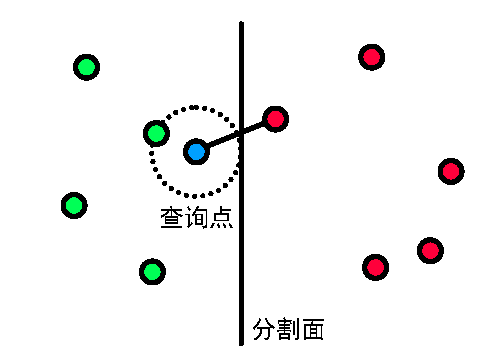
\includegraphics[width=0.4\textwidth]{resources/basic-point-cloud/kdtree-split-plane.pdf}
	\caption{Schematic of K-d tree pruning. In this figure, the distance from the splitting plane of the right branch exceeds the current nearest neighbor distance, indicating that points on the right must be farther than the current best solution. Thus, the right branch can be skipped.}
	\label{fig:kdtree-split-plane}
\end{figure}

Based on this principle, the nearest neighbor search in a K-d tree can be described as follows:

\begin{mdframed}
	\textbf{Nearest Neighbor Search in K-d Trees:}
	\begin{enumerate}
		\item \textbf{Input:} K-d tree \(T\), query point \(\bm{x}\).
		\item \textbf{Output:} Nearest neighbor of \(\bm{x}\).
		\item Let the current node be \(n_c\), initially the root node. Let \(d\) be the current minimum distance.
		\begin{enumerate}
			\item If \(n_c\) is a leaf, compute the distance between \(n_c\) and \(\bm{x}\). If it is smaller than \(d\), update \(n_c\) as the nearest neighbor and backtrack to its parent.
			\item If \(n_c\) is not a leaf, determine which side of \(n_c\) \(\bm{x}\) lies on. If the side containing \(\bm{x}\) has not been explored, prioritize exploring that side.
			\item Determine whether to explore the other side of \(n_c\). Compute the distance \(d'\) from \(\bm{x}\) to the splitting plane of \(n_c\). If \(d' < d\), the other side must be explored; otherwise, skip it.
			\item If both sides have been explored or need not be explored, backtrack to the parent node until \(n_c\) becomes the root node.
		\end{enumerate}
	\end{enumerate}
\end{mdframed}

For the \(k\)-nearest neighbor problem, the nearest neighbor becomes a set of points, and the distance threshold \(d\) is updated dynamically:

\begin{mdframed}
	\textbf{\(k\)-Nearest Neighbor Search in K-d Trees:}
	\begin{enumerate}
		\item \textbf{Input:} K-d tree \(T\), query point \(\bm{x}\), number of neighbors \(k\).
		\item \textbf{Output:} Set of \(k\)-nearest neighbors \(N\).
		\item Let the current node be \(n_c\), initially the root node. Define \(S(n_c)\) as the \(k\)-nearest neighbor search under \(n_c\):
		\begin{enumerate}
			\item If \(n_c\) is a leaf, compute its distance to \(\bm{x}\). If it is smaller than the largest distance in \(N\), add \(n_c\) to \(N\). If \(|N| > k\), remove the farthest point in \(N\).
			\item Determine which side of \(n_c\) \(\bm{x}\) lies on and recursively call \(S(n_c.\text{left})\) or \(S(n_c.\text{right})\).
			\item Determine whether to explore the other side of \(n_c\). The exploration condition is: if \(|N| < k\), explore; if \(|N| = k\) and the distance from \(\bm{x}\) to the splitting plane is less than the largest distance in \(N\), explore.
			\item If the other side need not be explored, return; otherwise, continue the search on the other side.
		\end{enumerate}
	\end{enumerate}
\end{mdframed}

In the worst case, this process may traverse the entire tree. If the query point lies near multiple splitting planes and the other side contains closer points, the K-d tree degenerates to linear search (brute-force), and its performance may even be worse due to the overhead of node traversal. The time complexity for searching a single nearest neighbor is logarithmic \(O(\log_2 N)\), while searching for \(k\) neighbors depends on the distribution of the point cloud. If the point cloud is well-distributed and the initial \(k\) neighbors are close, pruning can significantly reduce the search space. However, for large \(k\) or poorly distributed point clouds, more branches may need to be traversed.

In practice, it is often unnecessary to strictly find the exact \(k\)-nearest neighbors (e.g., if the \(k\)-th neighbor is much farther away). Thus, optimizations can be applied, such as setting a maximum number of points to visit or a timeout to terminate the search early. Another common optimization is to introduce a ratio \(\alpha\) for the pruning condition. Let \(d_{\text{max}}\) be the maximum distance in the current \(k\)-nearest neighbors and \(d_{\text{split}}\) be the distance to the splitting plane. If \(d_{\text{split}} > \alpha d_{\text{max}}\), the branch is pruned. Choosing \(\alpha \leq 1\) allows for more aggressive pruning.

\subsubsection{Implementation of K-d Tree Construction}
Below, we will briefly implement a K-d tree. While there are many open-source implementations of K-d trees, the teaching process often uses simpler and more understandable versions. We will first implement our own K-d tree and then compare it with the K-d tree in PCL, as well as with the algorithms mentioned earlier.

First, let's define the basic structure of the K-d tree. Each node contains pointers to its left and right children, as well as information about the splitting plane:

\begin{lstlisting}[language=c++, caption=src/ch5/kdtree.cc]
struct KdTreeNode {
	int id_ = -1;
	int point_idx_ = 0;            // Point index
	int axis_index_ = 0;           // Splitting axis
	float split_thresh_ = 0.0;     // Splitting threshold
	KdTreeNode* left_ = nullptr;   // Left subtree
	KdTreeNode* right_ = nullptr;  // Right subtree
	KdTreeNode* up_ = nullptr;     // Parent node
	
	bool IsLeaf() const { return left_ == nullptr && right_ == nullptr; }  // Whether it is a leaf
};
\end{lstlisting}

Each node stores the splitting axis and threshold. For example, if the splitting axis is the first axis (e.g., x-axis) and the threshold is 0.5, points with \(x < 0.5\) will be placed in the left subtree, while points with \(x \geq 0.5\) will be placed in the right subtree. Additionally, we record the ID of each node to facilitate indexing the tree without writing recursive code. Below are the basic member variables of the K-d tree:

\begin{lstlisting}[language=c++,caption=src/ch5/kdtree.h]
class KdTree {
	private:
	int k_ = 5;                                   // Number of nearest neighbors for KNN
	std::shared_ptr<KdTreeNode> root_ = nullptr;  // Root node
	std::vector<Vec3f> cloud_;                    // Input point cloud
	std::map<int, KdTreeNode*> nodes_;            // For bookkeeping
	size_t size_ = 0;                             // Number of leaf nodes
	int tree_node_id_ = 0;                        // Assigns IDs to K-d tree nodes
};
\end{lstlisting}

The K-d tree class holds a pointer to the root node, allowing traversal of the entire tree. We also maintain a map of node IDs to node pointers. Next, let's implement the tree construction process. Building the tree requires an input point cloud. We record the point cloud indices in the leaf nodes:

\begin{lstlisting}[language=c++,caption=src/ch5/kdtree.cc]
bool KdTree::BuildTree(const CloudPtr &cloud) {
	// Input validation code omitted
	IndexVec idx(cloud->size());
	for (int i = 0; i < cloud->points.size(); ++i) {
		idx[i] = i;
	}
	
	Insert(idx, root_.get());
	
	return true;
}

void KdTree::Insert(const IndexVec &points, KdTreeNode *node) {
	nodes_.insert({node->id_, node});
	
	if (points.empty()) {
		return;
	}
	
	if (points.size() == 1) {
		// Leaf node
		size_++;
		node->point_idx_ = points[0];
		return;
	}
	
	IndexVec left, right;
	FindSplitAxisAndThresh(points, node->axis_index_, node->split_thresh_, left, right);
	
	const auto create_if_not_empty = [&node, this](KdTreeNode *&new_node, const IndexVec &index) {
		if (!index.empty()) {
			new_node = new KdTreeNode;
			new_node->up_ = node;
			new_node->id_ = tree_node_id_++;
			
			Insert(index, new_node);
		}
	};
	
	create_if_not_empty(node->left_, left);
	create_if_not_empty(node->right_, right);
}

bool KdTree::FindSplitAxisAndThresh(const IndexVec &point_idx, int &axis, float &th, IndexVec &left, IndexVec &right) {
	// Calculate variance along each axis using functions from math_utils.h
	Vec3f var;
	Vec3f mean;
	math::ComputeMeanAndCovDiag(point_idx, mean, var, [this](const int &idx) { return cloud_[idx]; });
	int max_i, max_j;
	var.maxCoeff(&max_i, &max_j);
	axis = max_i;
	th = mean[axis];
	
	if (var.squaredNorm() < 1e-7) {
		// Edge case: All points have the same value. Split into left and right halves arbitrarily.
		// Rare in real data but possible in synthetic data.
		for (int i = 0; i < point_idx.size(); ++i) {
			if (i < point_idx.size() / 2) {
				left.emplace_back(point_idx[i]);
			} else {
				right.emplace_back(point_idx[i]);
			}
		}
		return true;
	}
	
	for (const auto &idx : point_idx) {
		if (cloud_[idx][axis] < th) {
			left.emplace_back(idx);
		} else {
			right.emplace_back(idx);
		}
	}
	
	if (point_idx.size() > 1) {
		// For non-trivial splits, ensure both subtrees are non-empty
		assert(left.empty() == false && right.empty() == false);
	}
	
	return true;
}
\end{lstlisting}

Here's the translation preserving all LaTeX commands exactly as in the original:

\subsection{Implementation of K-d Tree Construction}
The tree construction process is straightforward, implemented through recursive calls to the \texttt{Insert} function. If the input parameter \texttt{points} contains only one point, the current \texttt{node} becomes a leaf, and the point index is directly assigned. Otherwise, we calculate the variance along each axis, select the axis with the highest variance as the splitting axis, and use the mean value as the threshold. To handle edge cases where all points share identical coordinates (resulting in zero variance), we include a variance check.

Below is a test case for the tree construction process. We define four points on the \( z = 0 \) plane and observe the resulting tree structure:

\begin{lstlisting}[language=c++,caption=src/ch5/test\_nn.cc]
TEST(CH5_TEST, KDTREE_BASICS) {
	sad::CloudPtr cloud(new sad::PointCloudType);
	sad::PointType p1, p2, p3, p4;
	p1.x = 0; p1.y = 0; p1.z = 0;
	p2.x = 1; p2.y = 0; p2.z = 0;
	p3.x = 0; p3.y = 1; p3.z = 0;
	p4.x = 1; p4.y = 1; p4.z = 0;
	
	cloud->points.push_back(p1);
	cloud->points.push_back(p2);
	cloud->points.push_back(p3);
	cloud->points.push_back(p4);
	
	sad::KdTree kdtree;
	kdtree.BuildTree(cloud);
	kdtree.PrintAll();
	
	SUCCEED();
}
\end{lstlisting}

Compile and run the program:
\begin{lstlisting}[caption=Terminal input:]
bin/test_nn --gtest_filter=CH5_TEST.KDTREE_BASICS    
Note: Google Test filter = CH5_TEST.KDTREE_BASICS
[==========] Running 1 test from 1 test suite.
[----------] Global test environment set-up.
[----------] 1 test from CH5_TEST
[ RUN      ] CH5_TEST.KDTREE_BASICS
I0118 10:25:14.149652 295100 kdtree.cc:241] node: 0, axis: 0, th: 0.5
I0118 10:25:14.149777 295100 kdtree.cc:241] node: 1, axis: 1, th: 0.5
I0118 10:25:14.149780 295100 kdtree.cc:239] leaf node: 2, idx: 0
I0118 10:25:14.149780 295100 kdtree.cc:239] leaf node: 3, idx: 2
I0118 10:25:14.149781 295100 kdtree.cc:241] node: 4, axis: 1, th: 0.5
I0118 10:25:14.149782 295100 kdtree.cc:239] leaf node: 5, idx: 1
I0118 10:25:14.149783 295100 kdtree.cc:239] leaf node: 6, idx: 3
[       OK ] CH5_TEST.KDTREE_BASICS (0 ms)
\end{lstlisting}

\begin{figure}[!htp]
	\centering
	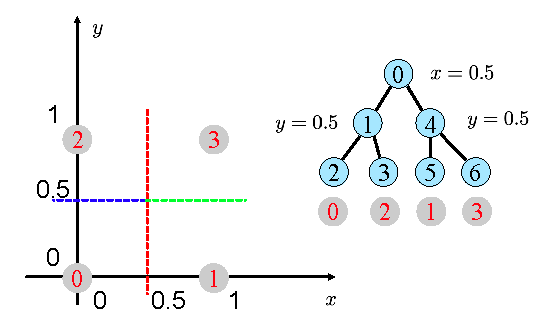
\includegraphics[width=0.8\textwidth]{resources/basic-point-cloud/kdtree-example.pdf}
	\caption{Schematic of the K-d tree construction for this example. Gray circles show point cloud IDs, while blue circles indicate K-d tree node IDs.}
	\label{fig:kdtree-example}
\end{figure}

The experimental results are illustrated in Figure~\ref{fig:kdtree-example}, displaying the splitting thresholds and leaf node information of the K-d tree. The constructed tree for these four points has two levels, with each splitting plane positioned at the midpoint between two points. Notably, since each split divides the remaining point cloud into two equal subsets, this K-d tree remains balanced, avoiding significant imbalance between left and right subtrees.  

Key observations:
1. \textbf{Axis Selection}: The first split occurs along the x-axis (axis 0) at \( x = 0.5 \), separating points \( p1, p3 \) (left) from \( p2, p4 \) (right).  
2. \textbf{Recursive Splitting}: Each subset is further split along the y-axis (axis 1) at \( y = 0.5 \), resulting in four leaf nodes.  
3. \textbf{Balance}: The tree depth is minimized due to equal partitioning, ensuring optimal search performance.  

This example demonstrates how K-d trees adaptively partition space based on data distribution, a property critical for efficient nearest neighbor searches in higher-dimensional datasets. The balance achieved here is a direct consequence of uniform point spacing, though real-world data may require additional balancing techniques (e.g., median-based splits) to maintain efficiency.

\subsubsection{Implementing K-Nearest Neighbors in K-d Trees}
Now let's implement the K-nearest neighbors (KNN) algorithm for K-d trees. When \(K=1\), this naturally becomes the nearest neighbor algorithm, so we don't need to implement a separate nearest neighbor search. First, we define a structure to record nodes and distances, along with its sorting method:

\begin{lstlisting}[language=c++,caption=src/ch5/kdtree.h]
/// For recording KNN results
struct NodeAndDistance {
	NodeAndDistance(KdTreeNode* node, float dis2) : node_(node), distance2_(dis2) {}
	KdTreeNode* node_ = nullptr;
	float distance2_ = 0;  // Squared distance for comparison
	
	bool operator<(const NodeAndDistance& other) const { return distance2_ < other.distance2_; }
};
\end{lstlisting}

We then use a priority queue to manage the KNN results. This queue maintains order during insertion, making it suitable for storing nearest neighbor results. The K-d tree nearest neighbor search is implemented as follows:

\begin{lstlisting}[language=c++,caption=src/ch5/kdtree.cc]
/// Compute K nearest neighbors
bool KdTree::GetClosestPoint(const PointType &pt, std::vector<int> &closest_idx, int k) {
	if (k > size_) {
		LOG(ERROR) << "cannot set k larger than cloud size: " << k << ", " << size_;
		return false;
	}
	k_ = k;
	
	std::priority_queue<NodeAndDistance> knn_result;
	Knn(ToVec3f(pt), root_.get(), knn_result);
	
	// Sort and return results
	closest_idx.resize(knn_result.size());
	for (int i = closest_idx.size() - 1; i >= 0; --i) {
		// Insert in reverse order
		closest_idx[i] = knn_result.top().node_->point_idx_;
		knn_result.pop();
	}
	return true;
}

/// Search for nearest neighbors of pt under node and add to result queue
void KdTree::Knn(const Vec3f &pt, KdTreeNode *node, std::priority_queue<NodeAndDistance> &knn_result) const {
	if (node->IsLeaf()) {
		// If leaf, check if it can be inserted
		ComputeDisForLeaf(pt, node, knn_result);
		return;
	}
	
	// Determine which side pt falls on and prioritize searching that subtree
	// Then check if the other subtree needs to be searched
	KdTreeNode *this_side, *that_side;
	if (pt[node->axis_index_] < node->split_thresh_) {
		this_side = node->left_;
		that_side = node->right_;
	} else {
		this_side = node->right_;
		that_side = node->left_;
	}
	
	Knn(pt, this_side, knn_result);
	if (NeedExpand(pt, node, knn_result)) {  // Note: comparison is with current best
		Knn(pt, that_side, knn_result);
	}
}

void KdTree::ComputeDisForLeaf(const Vec3f &pt, KdTreeNode *node,
std::priority_queue<NodeAndDistance> &knn_result) const {
	// Compare with current results and insert if better than worst distance
	float dis2 = Dis2(pt, cloud_[node->point_idx_]);
	if (knn_result.size() < k_) {
		// Not enough results yet
		knn_result.push({node, dis2});
	} else {
		// Already have k results, compare with current worst
		if (dis2 < knn_result.top().distance2_) {
			knn_result.push({node, dis2});
			knn_result.pop();
		}
	}
}

bool KdTree::NeedExpand(const Vec3f &pt, KdTreeNode *node, std::priority_queue<NodeAndDistance> &knn_result) const {
	if (knn_result.size() < k_) {
		return true;
	}
	
	// Check splitting plane distance to see if better results might exist
	float d = pt[node->axis_index_] - node->split_thresh_;
	if ((d * d) < knn_result.top().distance2_) {
		return true;
	} else {
		return false;
	}
}
\end{lstlisting}

The nearest neighbor function recursively calls the Knn function to perform the search. For leaf nodes, it compares the node's distance with the worst distance in the current KNN results. If better, it inserts into the priority queue. The NeedExpand function determines whether to search the other subtree based on the splitting plane distance.

Let's test our K-d tree implementation. We compare against brute-force results for ground truth and benchmark against PCL's K-d tree:

\begin{lstlisting}[language=sh, caption=Terminal input:]
bin/test_nn --gtest_filter=CH5_TEST.KDTREE_KNN 
I0118 17:07:02.307432 318029 sys_utils.h:32] Method Kd Tree build avg time/calls: 4.34059/1 ms.
I0118 17:07:02.307545 318029 test_nn.cc:234] Kd tree leaves: 18869, points: 18869
I0118 17:07:03.029914 318029 sys_utils.h:32] Method Kd Tree 5NN multi-thread avg time/calls: 3.01146/1 ms.
I0118 17:07:03.030046 318029 test_nn.cc:65] truth: 93895, esti: 93895
I0118 17:07:04.396924 318029 test_nn.cc:93] precision: 1, recall: 1, fp: 0, fn: 0
I0118 17:07:04.396939 318029 test_nn.cc:246] building kdtree pcl
I0118 17:07:04.398665 318029 sys_utils.h:32] Method Kd Tree build avg time/calls: 1.68209/1 ms.
I0118 17:07:04.398671 318029 test_nn.cc:252] searching pcl
I0118 17:07:04.411710 318029 sys_utils.h:32] Method Kd Tree 5NN in PCL avg time/calls: 12.9858/1 ms.
I0118 17:07:04.411908 318029 test_nn.cc:65] truth: 93895, esti: 93895
I0118 17:07:05.779804 318029 test_nn.cc:93] precision: 1, recall: 1, fp: 0, fn: 0
I0118 17:07:05.779814 318029 test_nn.cc:274] done.
\end{lstlisting}

The K-d tree achieves perfect precision and recall (100\%). Compared to PCL's implementation, our K-d tree takes longer to build (likely due to maintaining an additional node list) but demonstrates faster concurrent nearest neighbor searches.

\subsubsection{Implementing K-d Tree Construction and Nearest Neighbor Search}  

Through code implementation, we observe that the most critical part of the K-d tree nearest neighbor algorithm is **pruning**, and the pruning condition is that no closer nearest neighbor exists on the other side of the tree structure. Let the current farthest nearest neighbor distance be $d_{max}$, and the splitting plane distance be $d_{split}$. The pruning criterion can then be expressed as:  
\begin{equation}\label{key}  
	d_{split} > d_{max}.  
\end{equation}  

However, in the worst-case scenario, if the current nearest neighbor found is poor, we might need to search distant branches for a potentially closer neighbor. This is a situation we wish to avoid. Therefore, we can slightly modify the above criterion by introducing a scaling factor $\alpha$:  
\begin{equation}\label{key}  
	d_{split} > \alpha d_{max}.  
\end{equation}  

When $\alpha < 1$, the pruning condition is relaxed, making the K-nearest neighbor search faster, but we no longer guarantee finding the **exact nearest neighbor** (since their branches may have been pruned). This approach is referred to as **Approximate Nearest Neighbor (ANN)**. The ANN problem is more flexible than the KNN problem, allowing for various algorithmic and data structure approximations. In our code, we implement it as follows:  

\begin{lstlisting}[language=c++,caption=src/ch5/kdtree.cc]  
bool KdTree::NeedExpand(const Vec3f &pt, KdTreeNode *node, std::priority_queue<NodeAndDistance> &knn_result) const {  
	if (knn_result.size() < k_) {  
		return true;  
	}  
	
	if (approximate_) {  
		float d = pt[node->axis_index_] - node->split_thresh_;  
		if ((d * d) < knn_result.top().distance2_ * alpha_) {  
			return true;  
		} else {  
			return false;  
		}  
	} else {  
		// Check the splitting plane distance to see if a closer neighbor exists  
		float d = pt[node->axis_index_] - node->split_thresh_;  
		if ((d * d) < knn_result.top().distance2_) {  
			return true;  
		} else {  
			return false;  
		}  
	}  
}  
\end{lstlisting}  

The performance of the K-d tree with approximate nearest neighbor enabled (with $\alpha=0.1$) is as follows:  
\begin{lstlisting}[caption=Terminal output:]  
I0118 17:31:41.829752 320541 sys_utils.h:32] Method Kd Tree build average call time/count: 4.34565/1 ms.  
I0118 17:31:41.829856 320541 test_nn.cc:227] Kd tree leaves: 18869, points: 18869  
I0118 17:31:42.553129 320541 sys_utils.h:32] Method Kd Tree 5NN multithreaded average call time/count: 2.10658/1 ms.  
I0118 17:31:42.553233 320541 test_nn.cc:65] truth: 93895, esti: 93895  
I0118 17:31:44.371816 320541 test_nn.cc:91] precision: 0.771319, recall: 0.771319, fp: 21472, fn: 21472  
I0118 17:31:44.371834 320541 test_nn.cc:239] building kdtree pcl  
I0118 17:31:44.373656 320541 sys_utils.h:32] Method Kd Tree build average call time/count: 1.80198/1 ms.  
I0118 17:31:44.373662 320541 test_nn.cc:244] searching pcl  
I0118 17:31:44.387229 320541 sys_utils.h:32] Method Kd Tree 5NN in PCL average call time/count: 13.5384/1 ms.  
I0118 17:31:44.387405 320541 test_nn.cc:65] truth: 93895, esti: 93895  
I0118 17:31:45.723769 320541 test_nn.cc:91] precision: 1, recall: 1, fp: 0, fn: 0  
I0118 17:31:45.723780 320541 test_nn.cc:266] done.  
\end{lstlisting}  

It can be seen that the approximate method leads to some decline in precision and recall, with both metrics dropping to around 0.77, but there is an improvement in search speed. Compared to the algorithms in the previous section, the K-d tree is significantly better than brute-force search but slower than 2D and 3D voxel-based methods. If construction time is considered, it is even slower. In terms of performance, the K-d tree allows tuning the $\alpha$ parameter, enabling a balance between speed and accuracy. In contrast, grid-based methods, while very fast, often struggle to achieve satisfactory recall rates.  

The K-d tree in this chapter is implemented recursively, making the code concise, but it may encounter stack overflow issues with extremely large point clouds. Readers can modify it to an iterative implementation. Additionally, there are many improved versions of the K-d tree, which we will not implement here. Interested readers can explore open-source K-d tree algorithms such as \cite{Cai2021} for comparison. Furthermore, to save space, we have omitted discussions on other topics, such as how to delete a point from a K-d tree, how to balance a K-d tree, etc. Readers interested in these aspects are encouraged to refer to relevant literature.

\subsection{Quadtree and Octree}  

The K-d tree methods introduced earlier use a binary tree as the basic data structure. However, can we have more branches beyond just binary trees? The answer is yes. In two-dimensional and three-dimensional spaces, we have two corresponding approaches: the **Quadtree** \cite{Samet1984} and the **Octree** \cite{Meagher1982, Shaffer1987}. If we do not partition space using grids, other tree-based methods can also be derived. Since these two approaches follow the same underlying principle—only differing in spatial dimensionality—we will discuss them together.  

In a quadtree, each node has four children, while in an octree, each node has eight. This naturally corresponds to physical space: a rectangle can be divided into four equal parts by its center, and a 3D cube can be split into eight equal parts. The parent node represents the larger rectangle/cube, and the child nodes represent the subdivided rectangles/cubes, forming the quadtree and octree structures. This structure inherently defines the rules for space partitioning. Therefore, similar to the K-d tree, we can construct a quadtree/octree model for a 2D/3D point cloud and use analogous methods to perform nearest neighbor searches. Due to their more uniform spatial partitioning, quadtrees and octrees can also be used to describe data covering an entire space, such as maps.  

\begin{figure}[!htp]  
	\centering  
	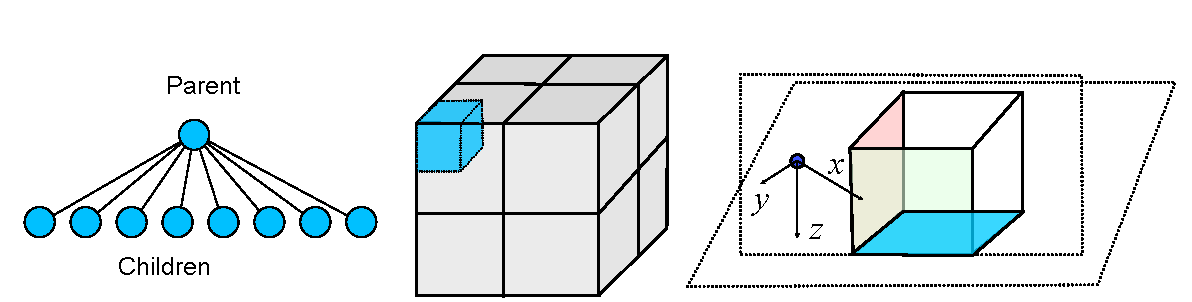
\includegraphics[width=1.0\textwidth]{resources/basic-point-cloud/octo-tree.pdf}  
	\caption{Schematic diagram of octree principles and distance computation. Left: The data structure of an octree; Middle: The partitioning method of an octree; Right: The distance calculation from an external point to a cube.}  
	\label{fig:octo-tree}  
\end{figure}

\subsubsection{Octree Construction}
Our focus is on 3D point cloud problems, so here we implement an octree algorithm, which also serves as a performance comparison experiment for readers. To maintain consistency, we try to mimic the K-d tree interface when implementing the octree, which also demonstrates their similarity. The main differences between octrees and K-d trees are:

\begin{enumerate}
	\item K-d trees use splitting planes to distinguish point sets, while octrees use cubic forms. For this purpose, we implemented a \texttt{Box3D} structure to handle the relationship between points and the octree.
	\item When building a K-d tree, the splitting planes are dynamically determined; in octrees, the subdivision of cubes is fixed (dividing into eight parts from the center). This means an octree node can always be expanded, but its child nodes may contain no point cloud. In this implementation, we retain those leaf nodes without corresponding point clouds. Of course, readers can choose to delete these leaf nodes, which would reduce the total number of nodes in the tree.
	\item During initial octree construction, we compute the bounding box of the entire point cloud as the root node's boundary box. This bounding box doesn't need to be a perfect cube. We allow it to be longer in certain dimensions, as long as subsequent subdivisions still follow the \textbf{eight-way split} rule. Readers can also enforce a perfect cube bounding box, but this may make the tree deeper and reduce search efficiency.
	\item The nearest neighbor search process in octrees is similar to K-d trees and also involves pruning. We use the \textbf{maximum perpendicular distance from the query point to the outer boundary of the bounding box} as the pruning criterion (see Figure~\ref{fig:octo-tree} for illustration). In this schematic, the query point is outside the grid in the x-direction but inside in the y and z directions. Therefore, the lower bound for the distance between the query point and the point cloud inside the cube should be the distance in the x-direction. If two or three axes are outside the cube, the longest axis should be taken as the distance lower bound. Readers can visualize this themselves. Of course, this lower bound could be estimated more precisely (e.g., by calculating the distance between the query point and the eight vertices of the cube), but we should ensure the distance calculation method is as simple as possible while maintaining effective pruning.
\end{enumerate}

With these differences in mind, we describe the octree construction and search algorithms:

\begin{mdframed}
	\textbf{Octree Construction:}
	\begin{enumerate}
		\item Input: Point cloud data $\bm{X} = \{\bm{x}_1, \ldots, \bm{x}_n\}$, where $\bm{x}_i \in \mathbb{R}^{k}$.
		\item Consider inserting subset $\bm{X}_n \subseteq \bm{X}$ into node $n$:
		\item If $\bm{X}_n$ is empty, exit;
		\item If $\bm{X}_n$ contains only one point, mark it as a leaf node and exit;
		\item Expand $n$ following the \textbf{eight-way split} rule.
		\item For each $\bm{x} \in \bm{X}_n$, record which child node contains $\bm{x}$. Then recursively apply the construction method to the child node and its corresponding point cloud.
		\item Repeat the above steps until all points are inserted into the tree.
	\end{enumerate}
\end{mdframed}

\subsubsection{Octree Search}
The k-nearest neighbor search algorithm for octrees can also be obtained by slightly modifying the K-d tree approach:

\begin{mdframed}
	\textbf{Octree k-Nearest Neighbor Search:}
	\begin{enumerate}
		\item Input: Octree $T$, query point $\bm{x}$, number of neighbors $k$;
		\item Output: k-nearest neighbor set $N$;
		\item Let the current node be $n_c$ (initially the root node). Define function $S(n_c)$ as performing k-nearest neighbor search under $n_c$:
		\begin{enumerate}
			\item If $n_c$ is a leaf, calculate whether the distance between $n_c$ and $\bm{x}$ is smaller than the maximum distance in $N$; if so, add $n_c$ to $N$. If $|N| > k$, remove the farthest matching point from $N$;
			\item Determine which child node of $n_c$ contains $\bm{x}$. If $\bm{x}$ is outside $n_c$'s bounding box, expand all child nodes; if inside, prioritize expanding the child node containing $\bm{x}$.
			\item Determine whether to expand other child nodes of $n_c$. The expansion condition: if $|N|<k$, expansion is mandatory; if $|N|=k$ and the previously calculated distance between $\bm{x}$ and $n_c$ is less than the maximum matching distance in $N$, also expand;
			\item If $n_c$'s child nodes don't need expansion, return; otherwise, continue calling the neighbor search algorithm for other nodes.
		\end{enumerate}
	\end{enumerate}
\end{mdframed}

\subsubsection{Code Implementation}  
Now let's implement the octree described earlier. An octree node consists of its bounding box and eight child nodes, defined as follows:

\begin{lstlisting}[language=c++,caption=src/ch5/octo\_tree.h]
struct Box3D {
	Box3D() = default;
	Box3D(float min_x, float max_x, float min_y, float max_y, float min_z, float max_z)
	: min_{min_x, min_y, min_z}, max_{max_x, max_y, max_z} {}
	
	float min_[3] = {0};
	float max_[3] = {0};
};

/// Octree node
struct OctoTreeNode {
	int id_ = -1;
	int point_idx_ = -1;                    // Point index, -1 means invalid
	bool box_set_ = false;                  // Whether bounding box is set
	Box3D box_;                             // Bounding box
	OctoTreeNode* children[8] = {nullptr};  // Child nodes
	OctoTreeNode* parent_ = nullptr;        // Parent node
};
\end{lstlisting}

Each bounding box consists of minimum and maximum values along three axes. The actual code also implements its distance calculation functions, which we won't show entirely here. Now let's look at the tree construction code:

\begin{lstlisting}[language=c++,caption=src/ch5/octo\_tree.cc]
bool OctoTree::BuildTree(const CloudPtr &cloud) {
	// Some validation code omitted	
	// Generate root node's bounding box
	root_->SetBox(ComputeBoundingBox());
	Insert(idx, root_.get());
	return true;
}

void OctoTree::Insert(const IndexVec &points, OctoTreeNode *node) {
	nodes_.insert({node->id_, node});
	
	if (points.empty()) {
		return;
	}
	
	if (points.size() == 1) {
		size_++;
		node->point_idx_ = points[0];
		return;
	}
	
	/// Continue expanding this node as long as point count isn't 1
	std::vector<IndexVec> children_points;
	ExpandNode(node, points, children_points);
	
	/// Perform insertion for child nodes
	for (size_t i = 0; i < 8; ++i) {
		Insert(children_points[i], node->children[i]);
	}
}

void OctoTree::ExpandNode(OctoTreeNode *node, const IndexVec &parent_idx, std::vector<IndexVec> &children_idx) {
	children_idx.resize(8);
	for (int i = 0; i < 8; ++i) {
		node->children[i] = new OctoTreeNode();
		node->children[i]->parent_ = node;
		node->children[i]->id_ = tree_node_id_++;
	}
	
	const Box3D &b = node->box_;  // Current node's box
	// Center point
	float c_x = 0.5 * (node->box_.min_[0] + node->box_.max_[0]);
	float c_y = 0.5 * (node->box_.min_[1] + node->box_.max_[1]);
	float c_z = 0.5 * (node->box_.min_[2] + node->box_.max_[2]);
	
	// Schematic of 8 sub-boxes
	// First layer: top-left 1, top-right 2, bottom-left 3, bottom-right 4
	// Second layer: top-left 5, top-right 6, bottom-left 7, bottom-right 8
	//     ---> x    /-------/-------/|
	//    /|        /-------/-------/||
	//   / |       /-------/-------/ ||
	//  y  |z      |       |       | /|
	//             |_______|_______|/|/
	//             |       |       | /
	//             |_______|_______|/
	node->children[0]->SetBox({b.min_[0], c_x, b.min_[1], c_y, b.min_[2], c_z});
	node->children[1]->SetBox({c_x, b.max_[0], b.min_[1], c_y, b.min_[2], c_z});
	node->children[2]->SetBox({b.min_[0], c_x, c_y, b.max_[1], b.min_[2], c_z});
	node->children[3]->SetBox({c_x, b.max_[0], c_y, b.max_[1], b.min_[2], c_z});
	
	node->children[4]->SetBox({b.min_[0], c_x, b.min_[1], c_y, c_z, b.max_[2]});
	node->children[5]->SetBox({c_x, b.max_[0], b.min_[1], c_y, c_z, b.max_[2]});
	node->children[6]->SetBox({b.min_[0], c_x, c_y, b.max_[1], c_z, b.max_[2]});
	node->children[7]->SetBox({c_x, b.max_[0], c_y, b.max_[1], c_z, b.max_[2]});
	
	// Assign points to child nodes
	for (const auto &idx : parent_idx) {
		const auto pt = cloud_[idx];
		for (int i = 0; i < 8; ++i) {
			if (node->children[i]->box_.Inside(pt)) {
				children_idx[i].emplace_back(idx);
				break;
			}
		}
	}
}
\end{lstlisting}

Special attention should be paid to the calculation order of width, height and depth in child node bounding boxes. Without the schematic diagram, mistakes can easily occur. Similar to K-d trees, we start from the root node and recursively call the Insert function to insert all point clouds into the octree. Note that once an octree node is expanded, it must have eight child nodes, even if there are fewer than eight points. Such an octree may contain some empty leaf nodes.

\subsubsection{K-Nearest Neighbor Search Implementation}
Now let's implement the K-nearest neighbor search. The algorithm logic is very similar to the K-d tree, with only a few key differences to note:

\begin{lstlisting}[language=c++,caption=src/ch5/octo\_tree.cc]
bool OctoTree::GetClosestPoint(const PointType &pt, std::vector<int> &closest_idx, int k) const {
	if (k > size_) {
		LOG(ERROR) << "cannot set k larger than cloud size: " << k << ", " << size_;
		return false;
	}
	
	std::priority_queue<NodeAndDistanceOcto> knn_result;
	Knn(ToVec3f(pt), root_.get(), knn_result);
	
	// Sort and return results
	closest_idx.resize(knn_result.size());
	for (int i = closest_idx.size() - 1; i >= 0; --i) {
		// Insert in reverse order
		closest_idx[i] = knn_result.top().node_->point_idx_;
		knn_result.pop();
	}
	return true;
}

void OctoTree::Knn(const Vec3f &pt, OctoTreeNode *node, std::priority_queue<NodeAndDistanceOcto> &knn_result) const {
	if (node->IsLeaf()) {
		if (node->point_idx_ != -1) {
			// For leaf nodes, check if the point is a nearest neighbor
			ComputeDisForLeaf(pt, node, knn_result);
			return;
		}
		return;
	}
	
	// Determine which cell contains pt, prioritize searching that subtree
	// Then check if other subtrees need searching
	// If pt is outside, prioritize the nearest subtree
	int idx_child = -1;
	float min_dis = std::numeric_limits<float>::max();
	for (int i = 0; i < 8; ++i) {
		if (node->children[i]->box_.Inside(pt)) {
			idx_child = i;
			break;
		} else {
			float d = node->box_.Dis(pt);
			if (d < min_dis) {
				idx_child = i;
				min_dis = d;
			}
		}
	}
	
	// First check idx_child
	Knn(pt, node->children[idx_child], knn_result);
	
	// Then check others
	for (int i = 0; i < 8; ++i) {
		if (i == idx_child) {
			continue;
		}
		
		if (NeedExpand(pt, node->children[i], knn_result)) {
			Knn(pt, node->children[i], knn_result);
		}
	}
}

bool OctoTree::NeedExpand(const Vec3f &pt, OctoTreeNode *node,
std::priority_queue<NodeAndDistanceOcto> &knn_result) const {
	if (knn_result.size() < k_) {
		return true;
	}
	
	if (approximate_) {
		float d = node->box_.Dis(pt);
		if ((d * d) < knn_result.top().distance_ * alpha_) {
			return true;
		} else {
			return false;
		}
	} else {
		// Without FLANN, perform normal search
		float d = node->box_.Dis(pt);
		if ((d * d) < knn_result.top().distance_) {
			return true;
		} else {
			return false;
		}
	}
}
\end{lstlisting}

Since each node has more branches, the code involves more loop traversals compared to the binary branching of K-d trees. Additionally, note that nearest neighbor points may not necessarily lie inside octree cells - they can be outside. When query points fall outside an octree cell, we prioritize expanding subtrees closer to the query point rather than following numerical order.

Below are the performance metrics and nearest neighbor evaluation results for our octree implementation:

\begin{lstlisting}[language=sh, caption=Terminal output:]
bin/test_nn --gtest_filter=CH5_TEST.OCTREE_KNN 
I0119 16:29:34.406015 343713 sys_utils.h:32] Method Octo Tree build average call time/count: 18.802/1 ms.
I0119 16:29:34.406155 343713 test_nn.cc:320] Octo tree leaves: 18869, points: 18869
I0119 16:29:34.406157 343713 test_nn.cc:323] testing knn
I0119 16:29:34.414115 343713 sys_utils.h:32] Method Octo Tree 5NN multithreaded average call time/count: 7.95114/1 ms.
I0119 16:29:34.414139 343713 test_nn.cc:328] comparing with bfnn
I0119 16:29:35.099203 343713 test_nn.cc:65] truth: 93895, esti: 93895
I0119 16:29:36.522886 343713 test_nn.cc:91] precision: 1, recall: 1, fp: 0, fn: 0
I0119 16:29:36.522902 343713 test_nn.cc:334] done.
\end{lstlisting}

Without using approximate nearest neighbor (ANN), the octree can find exact K-nearest neighbors. We've also implemented ANN parameters that readers can experiment with. Overall, due to the increased number of child nodes and more complex splitting plane calculations compared to K-d trees, the octree's construction time and KNN search time are slower than our custom K-d tree implementation (though still faster than PCL's K-d tree). When enabling ANN, the octree's performance improves, but at the cost of not achieving 100% precision and recall.

\subsection{Other Tree-Based Methods}
In practice, indexing spatial data to achieve fast neighborhood queries is an ancient and widespread problem. Beyond SLAM, we can find its applications in many other fields. Both closely related and distant domains—including \textbf{pattern recognition}, \textbf{classification}, \textbf{computer vision}, \textbf{coding theory}, \textbf{recommendation systems}, \textbf{speech recognition}, \textbf{chemistry}, \textbf{biology}, and others—all involve nearest neighbor problems \cite{Haining2003}.  

In SLAM, we focus on \textbf{low-dimensional} data structures that can be \textbf{quickly constructed and queried}, thus favoring simpler models. We also expect these structures to adapt rapidly to changes, such as adding new point clouds to the map, meaning K-d trees or octrees must support dynamic updates. In other applications, however, people deal with high-dimensional structured data (e.g., user demographics), tolerate longer construction times, but demand faster query speeds, giving rise to various \textbf{spatial data indexing} techniques. Many databases already support spatial data indexing. Broadly speaking, spatial indexing methods can be categorized as follows:

\begin{enumerate}
	\item \textbf{Tree- and forest-based spatial partitioning methods}:  
	- Ball trees \cite{Omohundro1989, Dolatshah2015, Liu2006}  
	- R-trees \cite{Guttman1984}  
	- R$^*$-trees \cite{Beckmann1990}  
	- Randomized K-d trees \cite{Duch1998}  
	- AABB trees \cite{Bergen1997}, etc.  
	While tree variants are extremely diverse, most share similar principles, differing mainly in spatial partitioning strategies\footnote{Back in the 1990s, proposing one's own improved algorithm was quite straightforward.}. For example, ball trees partition data using hyperspheres to ensure disjoint subtrees, while R-trees use minimum bounding boxes (MBBs) to organize data, and AABB trees follow a similar approach but are more commonly used in collision detection.
	
	\item \textbf{Space-filling curves}:  
	- Hilbert curves \cite{Lawder2001, Khoshgozaran2007}  
	- Z-order curves \cite{Orenstein1988}, etc.  
	These methods employ fractal curves to map high-dimensional spaces to one dimension while preserving locality, enabling efficient high-dimensional searches in lower dimensions.
	
	\item \textbf{Locality-Sensitive Hashing (LSH)} \cite{Datar2004, Teschner2003}:  
	LSH operates inversely to space-filling curves, hashing high-dimensional data into a lower-dimensional space while probabilistically preserving neighborhood relationships. In fact, our earlier grid-based methods already used such hashing to store grids—did you notice?
\end{enumerate}

Most spatial indexing methods mentioned here are better suited for \textbf{static, known datasets}. For instance, R-trees or R$^*$-trees are ideal for querying elements within a specific bounding box on a map. However, SLAM is inherently \textbf{dynamic}, requiring frequent creation and adjustment of point cloud maps, where constructing and destroying complex data structures can be time-consuming. Thus, SLAM tends to favor simpler, easily maintainable methods and often opts for approximate nearest neighbors over strict $k$-NN. Grids, voxels, and K-d trees remain the most preferred choices in SLAM.

We will not conduct comprehensive comparative experiments on these spatial indexing methods here. Readers may refer to survey literature \cite{Mahapatra2015, Bhatia2010} for performance comparisons or textbooks \cite{李航2012} for analyses of common spatial indexing algorithms.

\subsection{Summary}
This section introduced several common K-nearest neighbor (KNN) solutions in SLAM: brute-force search, grid-based methods, K-d trees, and octrees. As a summary, we present the performance comparison of these methods in Figure~\ref{fig:nn-compare} for reference. Typically, multithreaded implementations significantly outperform single-threaded ones. Readers may verify whether their experimental results align with ours.

\begin{figure}[!htp]
	\centering
	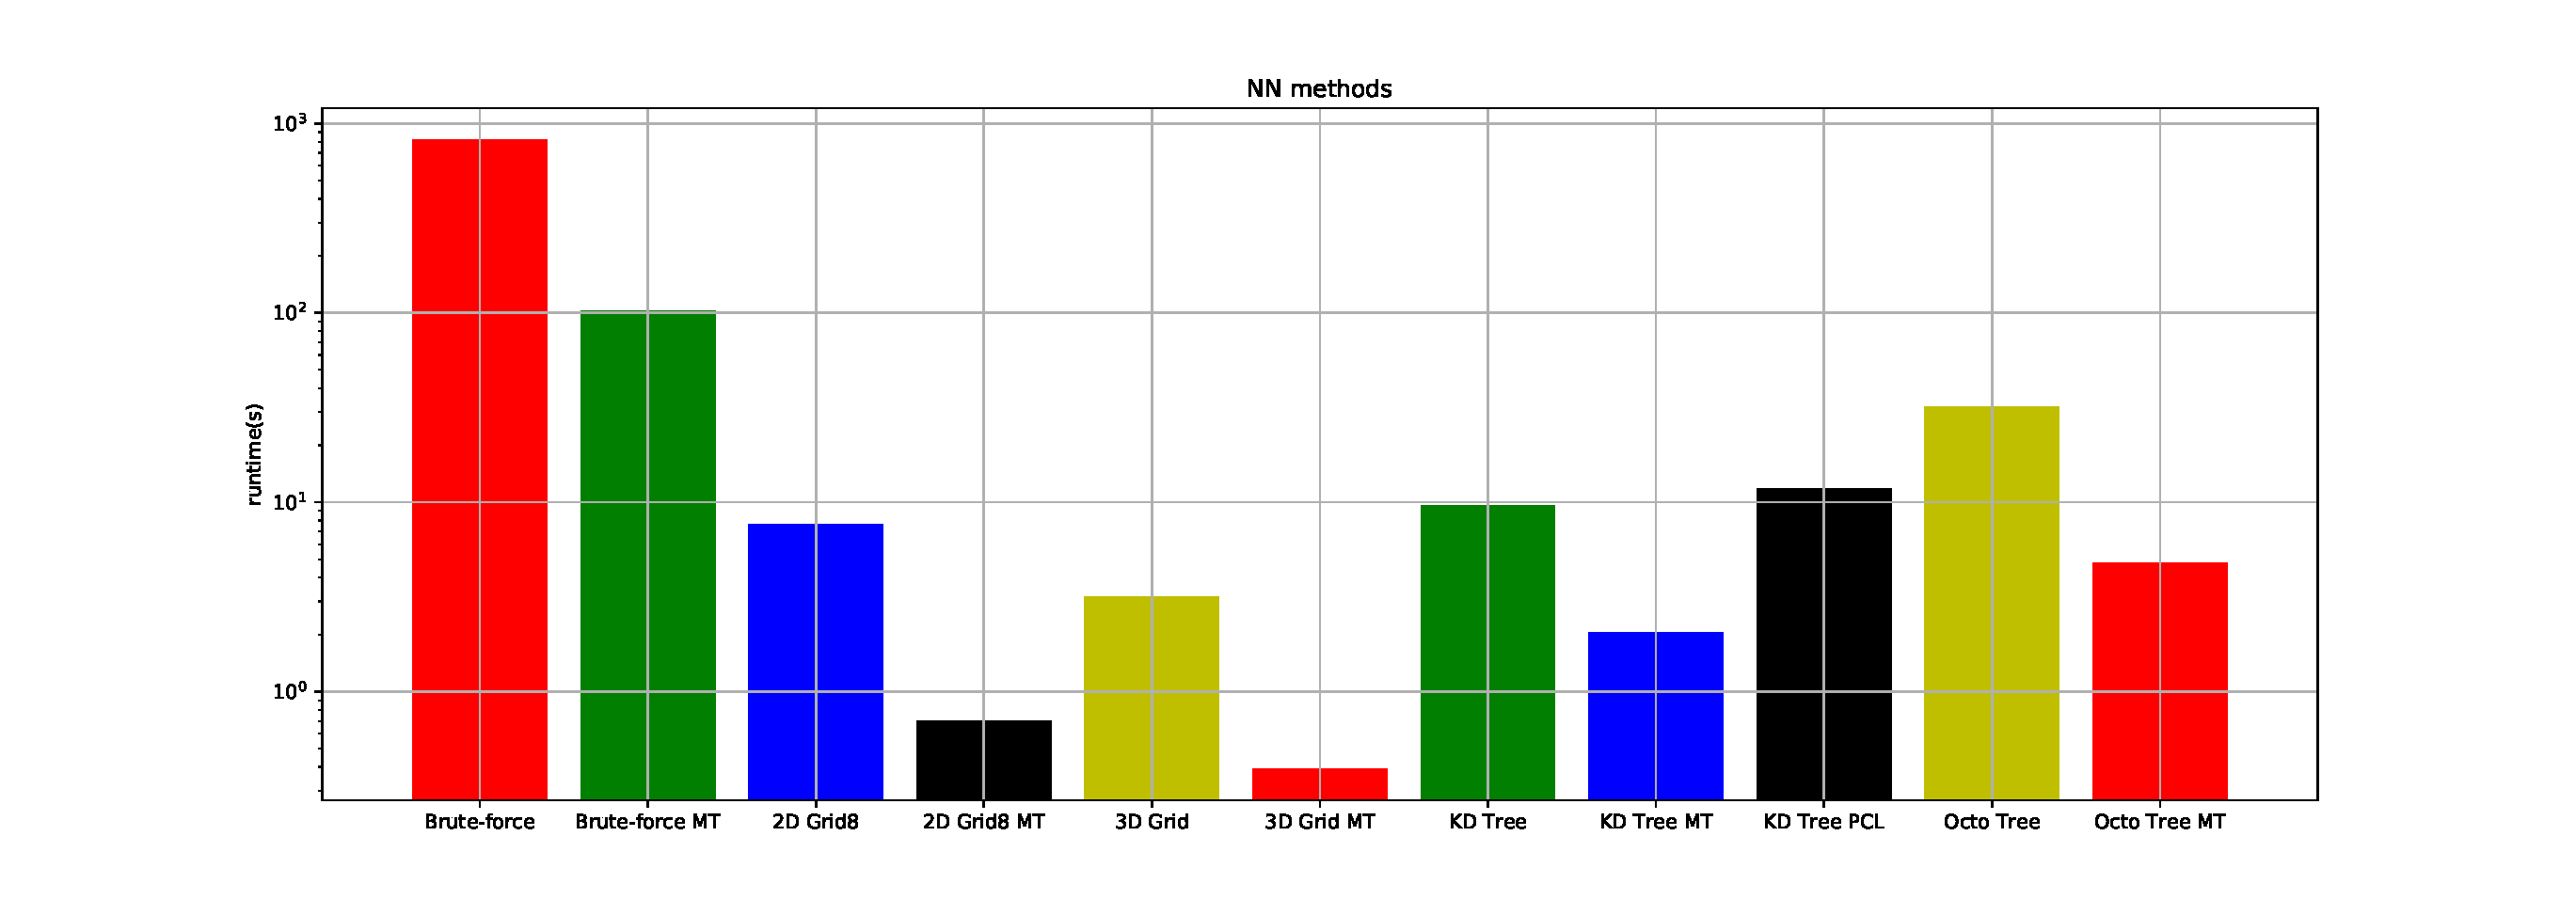
\includegraphics[width=1.0\textwidth]{resources/basic-point-cloud/nn-compare.pdf}
	\caption{Comparison of methods discussed in this section. From left to right: brute-force matching, multithreaded brute-force, 8-neighbor 2D grid, multithreaded 8-neighbor 2D grid, 3D voxel, multithreaded 3D voxel, KD-tree, multithreaded KD-tree, PCL's KD-tree, octree, and multithreaded octree. Note that due to the significantly longer computation time of brute-force matching, a logarithmic axis is used.}
	\label{fig:nn-compare}
\end{figure}

In terms of computation time, for our given dataset, 3D/2D grid-based methods performed the best, followed by K-d trees, while brute-force search was clearly the slowest. However, if the point cloud contains more points, the number of points within each grid cell will also increase, leading to linear growth in computational cost with grid cell density. Thus, grid methods are unsuitable for dense point clouds. In contrast, K-d trees exhibit logarithmic complexity growth. It can be inferred that beyond a certain scale, tree-based methods like K-d trees and octrees will become more advantageous. These tree-based approaches can also balance computation time and accuracy through approximate nearest neighbor (ANN) techniques.

\section{Fitting Problems}
Next, we introduce another important topic in point cloud processing algorithms: the extraction and estimation of basic geometric elements. Sometimes such problems are categorized as \textbf{detection} or \textbf{clustering} problems, leaning more towards perception methods. For example, many applications in autonomous driving focus heavily on extracting semantic elements like vehicles and pedestrians from point clouds. These elements can serve as data sources for subsequent decision-making and planning \cite{Navarro-Serment2010}. In SLAM, however, we are more concerned with how to use these elements to assist in \textbf{registration} between point clouds. Therefore, in traditional SLAM applications, the elements we focus on are typically basic and static, rather than dynamic or semantic. Registering a point to a plane is relatively straightforward, but registering one vehicle to another requires significantly more work\footnote{Even though the algorithm for registering two vehicles likely still relies on basic point-to-point methods.}.

In registration problems, a common approach is to first use a nearest-neighbor structure to find several nearest neighbors for a point, then fit these neighbors to a fixed geometric shape. Finally, the vehicle's pose is adjusted so that the scanned LiDAR points align with these shapes. The previous section covered various solutions to the nearest-neighbor problem, while this section focuses on extracting linear features like lines and planes from point clouds. We will see that these can be elegantly unified under the same framework (linear least squares) and solved using linear algebra.

\subsection{Plane Fitting}
As with many other problems, \textbf{linear} problems are often the simplest cases. Linear fitting of point clouds is the most basic component. The linear fitting problem for point clouds can be approached from several perspectives, and comparing these viewpoints provides different insights. The same problem may be referred to by different names across fields, yet their solutions are deeply interconnected. A linear fitting problem might be called \textbf{linear regression} (regressing the parameters of a line) or \textbf{principal component analysis (PCA)} (analyzing the primary axes of a point cloud's distribution).

Let's first consider plane fitting. Given a point cloud $\bm{X} = \{ \bm{x}_1, \ldots, \bm{x}_n \}$ composed of $n$ points, where each point has 3D Euclidean coordinates $\bm{x}_k \in \mathbb{R}^3$, we seek plane parameters $\bm{n}, d$ such that:
\begin{equation}
	\forall k \in [1, n], \bm{n}^\top \bm{x}_k + d = 0,
\end{equation}
where $\bm{n} \in \mathbb{R}^3$ is the normal vector and $d \in \mathbb{R}$ is the intercept.

Clearly, this problem has four unknowns, while each point provides one equation. With multiple points, noise typically makes the system overdetermined and unsolvable. Thus, we often seek a least squares solution (Linear Least Square) to minimize the error:
\begin{equation}
	\min_{\bm{n}, d} \sum_{k=1}^{n} \| \bm{n}^\top \bm{x}_k + d \|_2^2.
\end{equation}
Using homogeneous coordinates can further simplify the problem. The homogeneous coordinates of a 3D point are four-dimensional, though in practice we simply append a 1:
\begin{equation}
	\tilde{\bm{x}} = [\bm{x}^\top, 1]^\top \in \mathbb{R}^4.
\end{equation}
Thus, $\tilde{\bm{n}} = [\bm{n}^\top, d]^\top \in \mathbb{R}^4$ is also a homogeneous vector, and the problem can be rewritten as:
\begin{equation}\label{eq.6.6}
	\min_{\tilde{\bm{n}}} \sum_{k=1}^{n} \| \tilde{\bm{x}}^\top_k \tilde{\bm{n}} \|_2^2.
\end{equation}
The subscript 2 denotes the L2-norm (standard Euclidean norm), and the superscript 2 indicates the squared sum of norms. This is a \textbf{summation-form} linear least squares problem, which can also be expressed in matrix form. Stacking all points into a matrix:
\begin{equation}
	\tilde{\bm{X}} = [\tilde{\bm{x}}_1, \ldots, \tilde{\bm{x}}_n],
\end{equation}
the summation can be omitted:
\begin{equation}
	\min_{\tilde{\bm{n}}} \| \tilde{\bm{X}}^\top \tilde{\bm{n}} \|_2^2.
\end{equation}

This is essentially solving a linear algebra problem: given any matrix $\bm{A}$ (not necessarily square), we seek a non-zero vector $\bm{x}$ that minimizes $\bm{A} \bm{x}$. Of course, if $\bm{x} = 0$, the product is trivially zero, but we want non-trivial solutions, so we impose $\bm{x} \neq 0$. Moreover, scaling $\bm{x}$ by a non-zero constant $k$ scales $\bm{A}\bm{x}$ by $k$ (and its squared norm by $k^2$). Thus, we disregard the magnitude of $\bm{x}$ and focus on its direction by enforcing $\|\bm{x}\|=1$.

For $\bm{A}$, we impose no constraints. In the point cloud plane extraction problem, $\bm{A}$ is an $\mathbb{R}^{n \times 4}$ matrix, and $\bm{x}$ is a unit vector in $\mathbb{R}^4$. We can then ask: for which $\bm{x}$ does $\bm{A}\bm{x}$ attain its maximum or minimum?

Next, we will first discuss how to solve such problems in general linear algebra before returning to the plane fitting problem. Moving from the abstract to the concrete is always easier.

\subsubsection{Various Solutions to Linear Least Squares}
\paragraph{Eigenvalue Solution}
Algebraically, linear least squares refers to finding $\bm{x}^* \in \mathbb{R}^n$ for a given matrix $\bm{A} \in \mathbb{R}^{m \times n}$ such that:
\begin{equation}\label{key}
	\bm{x}^* = \arg \min_{\bm{x}} \|\bm{A} \bm{x} \|^2_2 =  \arg \min_{\bm{x}} \bm{x}^\top \bm{A}^\top 
	\bm{A} \bm{x}, \quad \text{s.t.}, \| \bm{x} \| = 1.
\end{equation}

We observe that $\bm{A}^\top \bm{A}$ is a real symmetric matrix. According to linear algebra theory, real symmetric matrices can always be diagonalized via eigenvalue decomposition:
\begin{equation}\label{key}
	\bm{A}^\top \bm{A} = \bm{V} \boldsymbol{\Lambda} \bm{V}^{-1},
\end{equation}
where $\boldsymbol{\Lambda}$ is a diagonal matrix of eigenvalues, which we assume are arranged in descending order as $\lambda_1, \ldots, \lambda_n$. $\bm{V}$ is an orthogonal matrix whose column vectors $\bm{v}_1, \ldots, \bm{v}_n$ are the corresponding eigenvectors, forming an orthonormal basis. Any vector $\bm{x}$ can be expressed as a linear combination of this basis:
\begin{equation}\label{key}
	\bm{x} = \alpha_1 \bm{v}_1 + \ldots + \alpha_n \bm{v}_n.
\end{equation}

It follows that\footnote{Alternatively, from the eigenvector perspective: $\bm{A}^\top \bm{A} \bm{x} = \sum_{k=1}^{n} \alpha_k \lambda_k \bm{v}_k$, yielding the same result.}:
\begin{equation}\label{key}
	\bm{V}^{-1} \bm{x} = \bm{V}^\top \bm{x} = [\alpha_1, \ldots, \alpha_n]^\top. 
\end{equation}

Thus, the objective function becomes:
\begin{equation}\label{key}
	\| \bm{A} \bm{x} \|_2^2 = \sum_{k=1}^{n} \lambda_k \alpha_k^2,
\end{equation}
with the constraint $\| \bm{x} \| = 1$ implying $\alpha_1^2 + \ldots + \alpha_n^2 = 1$. Since the eigenvalues $\lambda_k$ are arranged in descending order, the minimum is achieved by setting $\alpha_1 = 0, \ldots, \alpha_{n-1} = 0, \alpha_n = 1$, i.e., $\bm{x}^* = \bm{v}_n$.

We conclude that the optimal solution to the linear least squares problem is the \textbf{eigenvector corresponding to the smallest eigenvalue}. Since this problem aims to solve $\bm{A} \bm{x} = \bm{0}$, it can also be referred to as the \textbf{null space solution}. Note that the eigenvalue decomposition is performed on $\bm{A}^\top \bm{A}$ rather than directly on $\bm{A}$ (as $\bm{A}$ may not be diagonalizable, whereas $\bm{A}^\top \bm{A}$, being real symmetric, is guaranteed to be diagonalizable).

\paragraph{Singular Value Solution}
The aforementioned problem can also be approached from another perspective using \textbf{Singular Value Decomposition (SVD)}. Since any matrix can be decomposed via SVD, we perform SVD on $\bm{A}$ to obtain:
\begin{equation}\label{key}
	\bm{A} = \bm{U} \boldsymbol{\Sigma} \bm{V}^\top,
\end{equation}
where $\bm{U}$ and $\bm{V}$ are orthogonal matrices, and $\boldsymbol{\Sigma}$ is a diagonal matrix called the \textbf{singular value matrix}, with its diagonal elements being the singular values of $\bm{A}$, typically arranged in descending order.  

Substituting the SVD result into the linear least squares problem, since $\bm{U}$ is orthogonal, it cancels out when computing the L2-norm. We observe that this approach is essentially equivalent to the eigenvalue method:
\begin{equation}\label{key}
	\bm{x}^\top \bm{A}^\top \bm{A} \bm{x} = \bm{x}^\top \bm{V} 
	\boldsymbol{\Sigma}^2 \bm{V}^\top \bm{x}.
\end{equation}

Thus, similar to the eigenvalue solution, we take $\bm{x}$ as the last column of $\bm{V}$. In fact, the relationship between the singular values of $\bm{A}$ and the eigenvalues of $\bm{A}^\top\bm{A}$ is well-documented in many matrix theory textbooks \cite{Magnus1998, ZhangXianDa2004}. Here, we take this opportunity to reintroduce this concept through a practical problem.  

Furthermore, fitting an $(N-1)$-dimensional hyperplane to points in $N$-dimensional space can also be viewed as solving the null space problem in least squares. In summary, to fit a plane to a set of points, we simply:  

\begin{enumerate}
\item Arrange all point coordinates into matrix $\bm{A}$,  
\item Compute the right singular vector corresponding to the smallest singular value of $\bm{A}$, or compute the eigenvector corresponding to the smallest eigenvalue of $\bm{A}^\top \bm{A}$.  
\end{enumerate}

Either approach yields the desired solution.

\subsection{Plane Fitting Implementation}
Let's now implement plane fitting starting from a point cloud. Most linear algebra operations can be handled using Eigen. We implement the plane fitting function in the common math library:

\begin{lstlisting}[language=c++,caption=src/common/math\_utils.h]
template <typename S>
bool FitPlane(std::vector<Eigen::Matrix<S, 3, 1>>& data, Eigen::Matrix<S, 4, 1>& plane_coeffs, double eps = 1e-2) {
	if (data.size() < 3) {
		return false;
	}
	
	Eigen::MatrixXd A(data.size(), 4);
	for (int i = 0; i < data.size(); ++i) {
		A.row(i).head<3>() = data[i].transpose();
		A.row(i)[3] = 1.0;
	}
	
	Eigen::JacobiSVD svd(A, Eigen::ComputeThinV);
	plane_coeffs = svd.matrixV().col(3);
	
	// check error eps
	for (int i = 0; i < data.size(); ++i) {
		double err = plane_coeffs.template head<3>().dot(data[i]) + plane_coeffs[3];
		if (err * err > eps) {
			return false;
		}
	}
	
	return true;
}
\end{lstlisting}

We use fast SVD decomposition, computing only the last column of the SVD result for matrix $\bm{A}$. After computation, we also verify the squared error against points doesn't exceed a preset threshold. Now let's write a test program that:

1. Takes randomly generated plane parameters as ground truth
2. Samples points on the plane 
3. Adds noise
4. Performs plane fitting:

\begin{lstlisting}[language=c++,caption=src/ch5/linear\_fitting.cc]
void PlaneFittingTest() {
	Vec4d true_plane_coeffs(0.1, 0.2, 0.3, 0.4);
	true_plane_coeffs.normalize();
	
	std::vector<Vec3d> points;
	
	// Generate simulated plane points randomly
	cv::RNG rng;
	for (int i = 0; i < FLAGS_num_tested_points_plane; ++i) {
		// Generate random point, compute 4th dimension, add noise, then normalize
		Vec3d p(rng.uniform(0.0, 1.0), rng.uniform(0.0, 1.0), rng.uniform(0.0, 1.0));
		double n4 = -p.dot(true_plane_coeffs.head<3>()) / true_plane_coeffs[3];
		p = p / (n4 + 1e-18);  // Prevent division by zero
		p += Vec3d(rng.gaussian(FLAGS_noise_sigma), rng.gaussian(FLAGS_noise_sigma), rng.gaussian(FLAGS_noise_sigma));
		
		points.emplace_back(p);
		
		// Verify point-to-plane error
		LOG(INFO) << "res of p: " << p.dot(true_plane_coeffs.head<3>()) + true_plane_coeffs[3];
	}
	
	Vec4d estimated_plane_coeffs;
	if (sad::math::FitPlane(points, estimated_plane_coeffs)) {
		LOG(INFO) << "estimated coeffs: " << estimated_plane_coeffs.transpose()
		<< ", true: " << true_plane_coeffs.transpose();
	} else {
		LOG(INFO) << "plane fitting failed";
	}
}
\end{lstlisting}

Now compile and run the test program to compare estimated plane parameters with ground truth:
\begin{lstlisting}[language=sh,caption=Terminal output:]
./bin/linear_fitting 
I0121 11:04:49.878834 208913 linear_fitting.cc:21] testing plane fitting
I0121 11:04:49.879319 208913 linear_fitting.cc:46] res of p: -0.00149684
I0121 11:04:49.879382 208913 linear_fitting.cc:46] res of p: -0.00221244
...
I0121 11:04:49.879462 208913 linear_fitting.cc:51] estimated coeffs: 0.186755 0.363656 0.546692 0.730757, true: 0.182574 0.365148 0.547723 0.730297
\end{lstlisting}

We can observe the difference between ground truth and estimated parameters is around 3 decimal places. Additionally, linear methods don't depend on initial values and work well even when plane point coordinates are far from the origin.

\subsection{Line Fitting}
\label{sec:line-fitting}
Let us now consider a problem very similar to plane fitting: line fitting. We still assume the point set $\bm{X}$ consists of $n$ 3D points. However, we can describe a straight line in several different ways, such as treating the line as the intersection of two planes, or using a point on the line plus a direction vector to define the line. The latter approach is more intuitive.

Let a point $\bm{x}$ on the line satisfy the equation:
\begin{equation}\label{key}
	\bm{x} = \bm{d} t + \bm{p},
\end{equation}
where $\bm{d}, \bm{p} \in \mathbb{R}^3$, $t \in \mathbb{R}$. Here, $\bm{d}$ is the direction vector of the line, satisfying $\|\bm{d}\| = 1$; $\bm{p}$ is a point on the line $l$, and $t$ is the line parameter. We aim to solve for $\bm{d}$ and $\bm{p}$, totaling 6 unknowns. Clearly, when the given point set is large, this remains an overdetermined system, requiring the construction of a least squares problem for solution.

For any point $\bm{x}_k$ not on $l$, we can use the Pythagorean theorem to compute the squared perpendicular distance from the point to the line:
\begin{equation}\label{key}
	f^2_k = \| \bm{x}_k - \bm{p}\|^2 - \| (\bm{x}_k-\bm{p})^\top \bm{d} \|^2 ,
\end{equation}
and then formulate the least squares problem to solve for $\bm{d}$ and $\bm{p}$:
\begin{equation}\label{key}
	(\bm{d},\bm{p})^* = \arg \min_{\bm{d}, \bm{p}} \sum_{k=1}^{n} f_k^2, \quad \text{s.t.} \|\bm{d}\|= 1.
\end{equation}
Since the error term for each point is already squared, we simply need to sum them.

Next, we separate the $\bm{d}$ and $\bm{p}$ components. First, consider $\frac{\partial f^2_k}{\partial \bm{p}}$:
\begin{align}\label{key}
	\frac{\partial f^2_k}{\partial \bm{p}} &= -2(\bm{x}_k - \bm{p}) + 2 \underbrace{(\bm{x}_k - \bm{p})^\top \bm{d}}_{\text{scalar, }=\bm{d}^\top (\bm{x}_k - \bm{p})} \bm{d}, \\
	&= (-2) (\bm{I} - \bm{d} \bm{d}^\top) (\bm{x}_k - \bm{p}).
\end{align}
Thus, the derivative of the overall objective function with respect to $\bm{p}$ is:
\begin{align}\label{key}
	\frac{\partial \sum_{k=1}^{n} f_k^2}{\partial \bm{p}} &= \sum_{k=1}^{n} (-2) (\bm{I} - \bm{d} \bm{d}^\top) (\bm{x}_k - \bm{p}), \\ 
	&= (-2) (\bm{I} - \bm{d} \bm{d}^\top) \sum_{k=1}^n (\bm{x}_k - \bm{p}).
\end{align}
To find the extremum of the least squares problem, set this equal to zero, yielding:
\begin{equation}
	\bm{p} = \frac{1}{n} \sum_{k=1}^n \bm{x}_k,
\end{equation}
indicating that $\bm{p}$ should be the centroid of the point cloud. Thus, we can first determine $\bm{p}$ and then consider $\bm{d}$. With $\bm{p}$ solved, let $\bm{y}_k = \bm{x}_k - \bm{p}$, treating $\bm{y}_k$ as known, and simplify the error term:
\begin{equation}\label{eq.6.24}
	f_k^2 = \bm{y}_k^\top \bm{y}_k - \bm{d}^\top \bm{y}_k \bm{y}_k^\top \bm{d}.
\end{equation}

Clearly, the first error term does not contain $\bm{d}$ and is unaffected by the choice of $\bm{d}$, so it can be omitted. Minimizing the second term is equivalent to maximizing its negation:
\begin{equation}\label{key}
	\bm{d}^* = \arg \max_{\bm{d}} \sum_{k=1}^{n} \bm{d}^\top \bm{y}_k\bm{y}_k^\top \bm{d} = \sum_{k=1}^{n} \| \bm{y}_k^\top \bm{d}\|_2^2.
\end{equation}
If we define:
\begin{equation}\label{key}
	\bm{A} = \begin{bmatrix}
		\bm{y}_1^\top \\
		\ldots \\
		\bm{y}_n^\top
	\end{bmatrix},
\end{equation}
then the problem becomes:
\begin{equation}\label{eq.6.33}
	\bm{d}^* = \arg \max_{\bm{d}} \| \bm{A} \bm{d} \|_2^2.
\end{equation}
This problem is still very similar to (\ref{eq.6.6}), except that we seek to \textbf{maximize} rather than \textbf{minimize}. For plane fitting, we minimized this problem; for line fitting, we maximize it. Following the previous discussion, taking $\bm{d}$ as the eigenvector corresponding to the smallest eigenvalue or singular value yields the minimizing solution; conversely, taking the eigenvector corresponding to the largest eigenvalue yields the maximizing solution. Thus, the solution to this problem should take $\bm{d}$ as the right singular vector corresponding to the largest singular value of $\bm{A}$, or the eigenvector corresponding to the largest eigenvalue of $\bm{A}^\top \bm{A}$.

\begin{figure}[!htp]
	\centering
	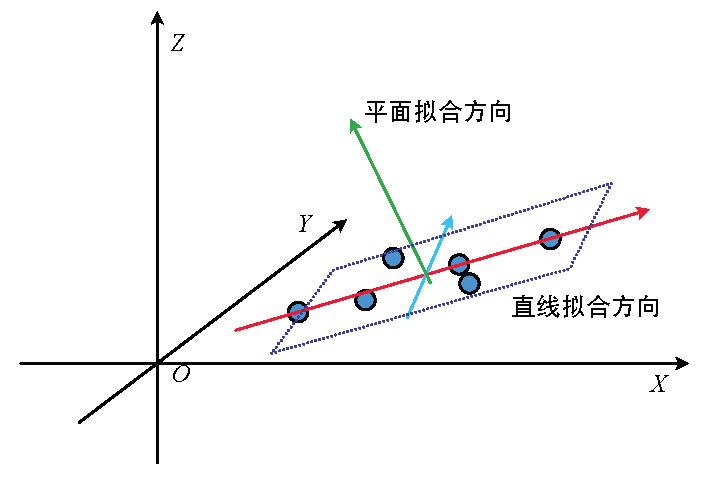
\includegraphics[width=0.5\textwidth]{resources/basic-point-cloud/linear-fitting.pdf}
	\caption{Schematic diagram of line fitting and plane fitting for point clouds (TODO: replace)}
	\label{fig:linear-fitting}
\end{figure}

\subsection{Implementation of Line Fitting}
Now let's implement the line fitting method described earlier. Similarly, we first implement the fitting function in the math library, then compare the fitted results with ground truth in a test program.

\begin{lstlisting}[language=c++,caption=src/common/math\_utils.h]
template <typename S>
bool FitLine(std::vector<Eigen::Matrix<S, 3, 1>>& data, Eigen::Matrix<S, 3, 1>& origin, Eigen::Matrix<S, 3, 1>& dir,
double eps = 0.2) {
	if (data.size() < 2) {
		return false;
	}
	
	origin = std::accumulate(data.begin(), data.end(), Eigen::Matrix<S, 3, 1>::Zero().eval()) / data.size();
	
	Eigen::MatrixXd Y(data.size(), 3);
	for (int i = 0; i < data.size(); ++i) {
		Y.row(i) = (data[i] - origin).transpose();
	}
	
	Eigen::JacobiSVD svd(Y, Eigen::ComputeFullV);
	dir = svd.matrixV().col(0);
	
	// check eps
	for (const auto& d : data) {
		if (dir.template cross(d - origin).template squaredNorm() > eps) {
			return false;
		}
	}
	
	return true;
}
\end{lstlisting}

Note that we need to compute the full $\bm{V}$ matrix of the SVD since we want the largest singular value. The rest of the computation remains consistent with the mathematical formulation. Below is the test program:

\begin{lstlisting}[language=c++,caption=src/ch5/linear\_fitting.cc]
void LineFittingTest() {
	// Ground truth line parameters
	Vec3d true_line_origin(0.1, 0.2, 0.3);
	Vec3d true_line_dir(0.4, 0.5, 0.6);
	true_line_dir.normalize();
	
	// Generate random points along the line using parametric equation
	std::vector<Vec3d> points;
	cv::RNG rng;
	for (int i = 0; i < fLI::FLAGS_num_tested_points_line; ++i) {
		double t = rng.uniform(-1.0, 1.0);
		Vec3d p = true_line_origin + true_line_dir * t;
		p += Vec3d(rng.gaussian(FLAGS_noise_sigma), rng.gaussian(FLAGS_noise_sigma), rng.gaussian(FLAGS_noise_sigma));
		
		points.emplace_back(p);
	}
	
	Vec3d esti_origin, esti_dir;
	if (sad::math::FitLine(points, esti_origin, esti_dir)) {
		LOG(INFO) << "estimated origin: " << esti_origin.transpose() << ", true: " << true_line_origin.transpose();
		LOG(INFO) << "estimated dir: " << esti_dir.transpose() << ", true: " << true_line_dir.transpose();
	} else {
		LOG(INFO) << "line fitting failed";
	}
}
\end{lstlisting}

Similarly, we first set the ground truth line parameters, add noise to sampled points along the line, then estimate the line parameters from these samples. The test results are:

\begin{lstlisting}[language=sh,caption=Terminal output:]
	./bin/linear_fitting
	I0121 12:14:10.936178 212707 linear_fitting.cc:24] testing line fitting
	I0121 12:14:10.936190 212707 linear_fitting.cc:77] estimated origin: 0.102906 0.204955 0.305633, true: 0.1 0.2 0.3
	I0121 12:14:10.936200 212707 linear_fitting.cc:78] estimated dir:  0.45294 0.569855 0.685646, true: 0.455842 0.569803 0.683763
\end{lstlisting}

At this point, we have demonstrated how to fit lines and planes to 3D point clouds. Interestingly, these two problems share remarkable similarities and can even be reduced to \textbf{finding the maximum and minimum solutions of the same problem}, as illustrated in Figure~\ref{fig:linear-fitting}. Line fitting seeks the direction of maximum variance, while plane fitting seeks the direction of minimum variance; line fitting corresponds to the eigenvector of the largest eigenvalue, while plane fitting corresponds to the smallest eigenvalue. This aligns perfectly with our intuition.

Extending to higher or lower dimensions, the plane fitting discussed here becomes fitting an $N-1$ dimensional hyperplane to points in $N$-dimensional space, while line fitting becomes fitting a 1-dimensional subspace. When points lie in 2D space ($N=2$), plane fitting reduces to line fitting, making the two problems identical. In higher dimensions, we can pose more complex questions - for example, what form should we fit for 5D point clouds in 4D or 3D space? While these questions may sound abstract, they have practical applications in numerous cases. Of course, people typically refer to them as \textbf{data} rather than point clouds. These $N-2$, $N-3$ dimensional fittings are also called \textbf{data dimensionality reduction}, implemented through SVD decomposition by selecting different columns of the $\bm{V}$ matrix or eliminating components with near-zero singular values while retaining those with larger singular values. Like squeezing water from a sponge, directions with small singular values represent \textbf{noise} while those with large singular values contain the \textbf{essential information}. These methods find applications in data compression, feature extraction, and more, with different names across domains. In Principal Component Analysis (PCA) \cite{Wold1987}, they're called \textbf{maximum principal components} or \textbf{minimum principal components}. In low-rank approximation problems \cite{Eckart1936}, line fitting can be viewed as a rank-1 approximation. Alternatively, in subspace analysis \cite{Lay2005}, line fitting constructs the range space (or row/column space) while plane fitting constructs the null space. Linear problems often exhibit intricate connections, with conclusions that are universally applicable. All these problems can be modeled as linear least squares problems, with SVD or eigenvalue decomposition remaining the core solution approaches.

\section{Summary}
This chapter introduced fundamental point cloud representations and basic point cloud-related problems, such as nearest neighbor search and fitting solutions. Starting from first principles, we implemented brute-force nearest neighbor search, K-d trees, octrees, and other nearest neighbor methods, and conducted comparative experiments with PCL versions in terms of efficiency and accuracy. Since we only need to consider LiDAR point clouds without accommodating various other point cloud templates, our implementations of K-d trees and other data structures are more concise than PCL's versions. These data structures are highly useful and will be employed in subsequent chapters to implement point cloud registration, odometry, and other algorithmic modules.

\section*{Exercises}
\begin{enumerate}
	\item Define NEARBY14 in 3D voxels and implement 14-cell nearest neighbor search.
	\item Extend the K-d tree point cloud type to a template class.
	\item Incorporate bounding boxes into the K-d tree node structure to achieve more precise pruning.
	\item Attempt to improve the lower bound accuracy of the distance between query points and bounding boxes in octrees, and observe whether nearest neighbor performance improves.
	\item Derive that the solution to Equation~\eqref{eq.6.33} is the eigenvector corresponding to the largest eigenvalue of $\bm{A}^\top \bm{A}$.
	\item Compare the nearest neighbor algorithms in this chapter with common approximate nearest neighbor algorithms such as nanoflann \cite{Blanco2014}, Faiss \cite{Johnson2019}, and nmslib \cite{Boytsov2016}, and evaluate their performance in point cloud nearest neighbor search.
\end{enumerate}